\section*{Supplementary materials}\label{supplementary-materials-table-of-contents}
\addcontentsline{toc}{section}{Supplementary materials}

\renewcommand{\thetable}{S\arabic{table}}
\renewcommand{\thefigure}{S\arabic{figure}}

\setcounter{page}{1}
\startcontents[appendix]
\printcontents[appendix]{}{1}{\setcounter{tocdepth}{2}}


\newpage

\section{Migration situation in
Poland}\label{sec-appen-migration-situation}

\subsection{Definitions}\label{sec-appen-definitions}

\subsubsection{Polish original version}\label{polish-original-version}

\textbf{Nielegalny pobyt} -- pobyt niezgodny z przepisami dotyczącymi
warunków wjazdu cudzoziemców na terytorium Rzeczypospolitej Polski i ich
pobytu na tym terytorium.

Nielegalny pobyt na terytorium RP ma miejsce w szczególności w sytuacji,
gdy cudzoziemiec:

\begin{itemize}
\tightlist
\item
  Nie posiada ważnej wizy lub innego ważnego dokumentu uprawniającego go
  do wjazdu na terytorium Rzeczypospolitej Polskiej i pobytu na nim.
\item
  Nie opuścił terytorium Rzeczypospolitej Polskiej po wykorzystaniu
  dopuszczalnego okresu pobytu.
\item
  Nielegalnie przekroczył lub usiłował nielegalnie przekroczyć granicę.
\item
  Nielegalnie wykonuje lub wykonywał pracę.
\item
  Podjął działalność gospodarczą niezgodnie z obowiązującymi przepisami.
\item
  Nie posiada wystarczających środków finansowych do pobytu na
  terytorium Rzeczypospolitej Polskiej.
\item
  Został zastrzeżony do celów odmowy wjazdu w SIS lub krajowym wykazie.
\end{itemize}

Głównym skutkiem prawnym nielegalnego pobytu jest wszczęcie postępowania
administracyjnego w celu \textbf{zobowiązania cudzoziemca do powrotu}
(deportacji). Stosuje się następujące środki:

\begin{itemize}
\tightlist
\item
  \textbf{Decyzje administracyjne:}

  \begin{itemize}
  \tightlist
  \item
    \textbf{Decyzja o powrocie:} Nakłada na cudzoziemca obowiązek
    opuszczenia Polski. Zazwyczaj wyznacza się termin dobrowolnego
    wyjazdu (od 15 do 30 dni).
  \item
    \textbf{Zakaz wjazdu:} Decyzji o powrocie towarzyszy zakaz ponownego
    wjazdu na terytorium RP oraz strefy Schengen na okres od 6 miesięcy
    do 5 lat.
  \item
    \textbf{Wpis do SIS:} Dane są wprowadzane do Systemu Informacyjnego
    Schengen, co skutkuje odmową wjazdu do większości krajów
    europejskich.
  \end{itemize}
\item
  \textbf{Zatrzymanie i środki przymusu:}

  \begin{itemize}
  \tightlist
  \item
    \textbf{Strzeżone ośrodki:} Sąd może nakazać umieszczenie
    cudzoziemca w strzeżonym ośrodku dla cudzoziemców w celu
    zabezpieczenia wykonania decyzji o powrocie.
  \item
    \textbf{Środki alternatywne:} Obowiązek zgłaszania się do organów
    Straży Granicznej, przekazanie dokumentu podróży do depozytu lub
    zabezpieczenie finansowe.
  \end{itemize}
\item
  \textbf{Odpowiedzialność finansowa i karna:}

  \begin{itemize}
  \tightlist
  \item
    \textbf{Grzywna:} Nielegalny pobyt stanowi wykroczenie podlegające
    karze grzywny.
  \item
    \textbf{Kara pozbawienia wolności:} Nielegalne przekroczenie granicy
    przy użyciu siły lub posługiwanie się fałszywymi dokumentami może
    skutkować odpowiedzialnością karną (od 3 do 8 lat więzienia).
  \end{itemize}
\item
  \textbf{Nieważność dokumentów:} Z dniem, w którym decyzja o powrocie
  staje się ostateczna, posiadane wizy lub zezwolenia na pracę wygasają
  z mocy prawa.
\end{itemize}

\subsubsection{English translation}\label{english-translation}

\textbf{Illegal stay (Poland)} -- stay not in accordance with the
regulations concerning the conditions of entry of foreigners into the
territory of the Republic of Poland and their stay in that territory.

Illegal stay on the territory of the Republic of Poland occurs in
particular when a foreigner:

\begin{itemize}
\tightlist
\item
  Does not have a valid visa or other valid document entitling him/her
  to enter and stay on the territory of the Republic of Poland.
\item
  Has not left the territory of the Republic of Poland after the expiry
  of the permitted period of stay.
\item
  Has illegally crossed or attempted to illegally cross the border.
\item
  Is or has been working illegally.
\item
  Has undertaken economic activity in violation of the applicable
  regulations.
\item
  Does not have sufficient financial means to stay in the territory of
  the Republic of Poland.
\item
  Has been flagged for refusal of entry in the SIS or national list.
\end{itemize}

The primary legal consequence of an illegal stay is the initiation of
administrative proceedings to \textbf{oblige the foreigner to return}
(deportation). The following measures are applied:

\begin{itemize}
\tightlist
\item
  \textbf{Administrative Decisions:}

  \begin{itemize}
  \tightlist
  \item
    \textbf{Order to Return:} A decision is issued requiring the
    foreigner to leave Poland. A period for voluntary departure (usually
    15--30 days) is typically granted.
  \item
    \textbf{Entry Ban:} Return decisions usually include a ban on
    re-entering Poland and the Schengen Area for a period of 6 months to
    5 years.
  \item
    \textbf{SIS Entry:} Data is recorded in the Schengen Information
    System, effectively blocking entry to most European countries.
  \end{itemize}
\item
  \textbf{Detention and Restrictive Measures:}

  \begin{itemize}
  \tightlist
  \item
    \textbf{Guarded Centres:} A court may order placement in a guarded
    centre for foreigners (detention) to ensure deportation.
  \item
    \textbf{Alternative Measures:} Requirement to report regularly to
    authorities, surrender of travel documents, or financial deposits.
  \end{itemize}
\item
  \textbf{Financial and Criminal Liability:}

  \begin{itemize}
  \tightlist
  \item
    \textbf{Fines:} Illegal stay is a misdemeanour punishable by a fine
    (\emph{grzywna}).
  \item
    \textbf{Imprisonment:} Crossing the border by force or using forged
    documents can lead to criminal prosecution and imprisonment (up to
    3--8 years depending on the offence).
  \end{itemize}
\item
  \textbf{Legal Invalidity:} Any existing visas or work permits are
  automatically invalidated the moment the return decision becomes
  final.
\end{itemize}


\subsection{Police records and unauthorised stay}\label{sec-appen-police}

The Police maintain the National Police Information System
(pol. \emph{Krajowy System Informacyjny Policji}, KSIP), which includes criminal records, person searches, process registrations, and traffic offences. 
We use the first and third, criminal
records (\emph{notowania kryminalne}) and process registrations
(\emph{rejestracja procesowa}), since both concern crime: process
registration records a~suspect or accused person in an offence prosecuted
\emph{ex officio}, entered during pre-trial proceedings, while a criminal
record links a person to a crime gathered in the course of police work.

Unauthorised stay is not such an offence but a petty offence under
Article~465 of the Act on Foreigners, adjudicated under the Code of
Procedure in Cases of Petty Offences and handled by the Border Guard, so
it appears in neither register. KSIP therefore records irregular migrants
only when they were also linked to a crime, and its overlap with the
Border Guard's within-country detections is small.

\clearpage


\subsection{Changes in the law regarding stay and
work}\label{sec-appen-changes-law}

\begin{table}[ht!]

\caption{\label{tbl-appen-stay-changes}Key legislative changes
concerning the legality and duration of stay of foreigners in Poland
(2020--2024).}

\centering{

\centering\begingroup\fontsize{7}{9}\selectfont

\begin{threeparttable}
\begin{tabular}{>{\raggedright\arraybackslash}p{1.2cm}>{\raggedright\arraybackslash}p{3.2cm}>{\raggedright\arraybackslash}p{4.8cm}>{\raggedright\arraybackslash}p{2.5cm}>{\raggedright\arraybackslash}p{3.2cm}}
\toprule
Year & Legal act & Document type & Extension mechanism & Group\\
\midrule
2020 & Act of 2 March 2020 (Dz.U. 2020 poz. 374, as amended) & National visas (D) & Automatic extension ex lege until 30 July 2023 & All third-country nationals\\
2020 & Same & Schengen visas issued by Poland & Legal stay extended on Polish territory until 30 July 2023 (no Schengen mobility) & All third-country nationals\\
2020 & Same & Visa-free stay (90/180 rule) & Period of stay considered legal until 30 July 2023 & All third-country nationals\\
2020 & Same & Temporary residence permits & Validity extended ex lege until 30 July 2023 & All third-country nationals\\
2020 & Same & Residence cards (temporary, permanent, EU long-term) & Expiry tolerated; stay remained legal despite formal expiry & All third-country nationals\\
\addlinespace
2020 & Same & Deadlines for residence permit applications & Administrative deadlines suspended during epidemic period & All third-country nationals\\
2020 & Same & Return decisions and obligation to leave & Suspension of deadlines for voluntary departure and enforcement & All third-country nationals\\
2022 & Act of 12 March 2022 (Dz.U. 2022 poz. 583) & Special protection status (UKR) & Legal stay for 18 months from 24 February 2022 & Ukrainian citizens\\
2022 & EU temporary protection (Dz.U. 2022 poz. 1383 et seq.) & Temporary protection extension & Protection extended until 4 March 2024 & Ukrainian citizens\\
2024 & EU Council Decision (Dz.U. 2024 poz. 232; 854) & Temporary protection extension & Protection extended until 4 March 2025 & Ukrainian citizens\\
\addlinespace
2023 & Amendment to Special Act on Ukraine (Dz.U. 2023 poz. 185) & Access to temp. residence after UKR stay & Temp. residence after 9 months of UKR status & Ukrainian citizens\\
\bottomrule
\end{tabular}
\begin{tablenotes}
\item \textit{Note: } 
\item COVID-related extensions applied ex lege and were valid until 30 days after the end of the epidemic threat state in Poland (1 July 2023). These measures regularised stay only on Polish territory and did not restore Schengen mobility rights.
\end{tablenotes}
\end{threeparttable}
\endgroup{}

}

\end{table}%

\clearpage

\begin{table}[ht!]

\caption{\label{tbl-appen-work-changes}Key legislative changes
concerning access to employment and duration of work authorisation for
foreigners in Poland (2020--2024).}

\centering{

\centering\begingroup\fontsize{7}{9}\selectfont

\begin{threeparttable}
\begin{tabular}{>{\raggedright\arraybackslash}p{1.2cm}>{\raggedright\arraybackslash}p{3.2cm}>{\raggedright\arraybackslash}p{4.8cm}>{\raggedright\arraybackslash}p{2.8cm}>{\raggedright\arraybackslash}p{3.2cm}}
\toprule
Year & Legal act & Work authorisation type & Extension / new duration & Group\\
\midrule
2020 & Act of 2 March 2020 (Dz.U. 2020 poz. 374, as amended) & Work permits (types A--E) & Validity extended until 30 July 2023 & Third-country nationals\\
2020 & Same & Employer declaration (oswiadczenie) & Continued work allowed despite expiry during epidemic & Citizens of UA, BY, MD, GE, AM, RU\\
2020 & Same & Seasonal work permits & Automatic extension until 30 July 2023 & Selected third-country nationals\\
2022 & Act of 17 Dec. 2021 (Dz.U. 2022 poz. 91) & Employer declaration system & Max duration extended from 6 to 24 months & Citizens of UA, BY, MD, GE, AM, RU\\
2022 & Special Act on Ukraine (Dz.U. 2022 poz. 583) & Access to labour market without work permit & Unrestricted access upon registration by employer & Ukrainian citizens\\
\addlinespace
2022 & Amendments to Foreigners Act & Single permit (residence and work) & Statutory 60-day deadline for completeness verification & Third-country nationals\\
2020--2023 & COVID-19 legislation (Act of 2 March 2020 et seq.) & Modification of employment conditions & Temporary permission to change conditions without amending permits & Third-country nationals\\
\bottomrule
\end{tabular}
\begin{tablenotes}
\item \textit{Note: } 
\item COVID-related provisions preserved the legal validity of existing work authorisations but did not create new permits. Extensions applied until 30 days after the end of the epidemic threat state in Poland (30 July 2023).
\end{tablenotes}
\end{threeparttable}
\endgroup{}

}

\end{table}%

\clearpage

\section{Border Guard and Police staffing and inspections
statistics}\label{sec-appen-more-on-border-guards}

Table \ref{tbl-appen-border-guard} reports annual staffing stocks and
enforcement outcomes for the Polish Border Guard and Police.

\begin{table}[H]

\caption{\label{tbl-appen-border-guard}Border Guard and Police staffing and enforcement inspection outcomes, 2019--2025}

\centering{


\begin{adjustbox}{max width=\textwidth}
\begin{threeparttable}

\begin{tabular}{lrrrrrrr}
\toprule
 & 2019 & 2020 & 2021 & 2022 & 2023 & 2024 & 2025 \\
\midrule
\multicolumn{8}{l}{\textit{Police Staffing}} \\[2pt]
\quad Total employment      & 98,820 & 97,899 & 100,557 & 101,000 & 96,698 & 97,256 & 102,288 \\
\quad Recruitments          &    4,655 &   4,373 &   6,684 &    5,169 &  5,174 &  6,411 & 8,509 \\
\quad Separations           &    4,567 &   5,234 &    4,053 &    4,726 &  9,457 &    -- &    -- \\
\midrule
\multicolumn{8}{l}{\textit{Border Guards Staffing}} \\[2pt]
\quad Total employment      & 14,718 & 14,496 & 14,845 & 15,098 & 14,858 & 15,488 & 16,557 \\
\quad Recruitments          &    409 &    426 &    767 &    869 &  1,098 &  1,389 &  1,449 \\
\quad Separations           &    544 &    648 &    418 &    616 &  1,338 &    759 &    380 \\
\midrule
\multicolumn{8}{l}{\textit{Employment legality verification}} \\[2pt]
\quad Inspections conducted [A]                        &  4,028 &  2,388 &  2,183 &  1,943 &  1,843 &  1,826 & 1,652 \\
\quad Foreigners verified [B]                          & 124,979 & 60,811 & 87,295 & 72,689 & 73,291 & 76,995 & 64,520 \\
\quad Illegally employed foreigners [C]                & 14,740 &  9,899 & 12,264 & 11,407 &  9,968 & 10,755 & 13,231 \\
\quad Foreigners per inspection [B/A]\tnote{a}         &   31.0 &   25.5 &   40.0 &   37.4 &   39.8 &   42.2 & 38.1 \\
\quad Illegal employment detection rate [C/B]\tnote{b} &   11.8 &   16.3 &   14.0 &   15.7 &   13.6 &   14.0 & 20.1 \\
\midrule
\multicolumn{8}{l}{\textit{Legality of stay verification}} \\[2pt]
\quad Inspections conducted [D]                        & 26,757 & 17,691 & 15,686 & 16,267 & 20,988 & 26,162 & 30,445 \\
\quad Foreigners verified [E]                          & 61,355 & 40,536 & 39,714 & 43,549 & 57,929 & 68,229 & 81,239 \\
\quad Illegally staying foreigners [F]                 & 11,153 & 5,823 & 9,490 & 6,984 & 11,152 & 13,935 & 13,377 \\
\quad Foreigners per inspection [E/D]\tnote{a}         &    2.3 &    2.3 &    2.5 &    2.7 &    2.8 &    2.6 &    2.7 \\
\quad Illegally staying detection rate [F/E]\tnote{b}  &   18.2 &   14.4 &   23.9 &   16.0 &   19.3 &   20.4 &   16.5 \\
\bottomrule
\end{tabular}
\begin{tablenotes}
\small
\item[a] Average number of foreigners verified per inspection;
\item[b] Share of illegally working/present foreigners among all verified, in \%.

The table reports annual staffing stocks and enforcement outcomes for the Polish Border Guard. Total employment refers to the headcount at year-end. Recruitments and separations refer to officers joining and leaving the service during the calendar year. Inspections conducted refers to the number of employer or entity premises visited. Foreigners verified refers to the total number of individual foreigners whose status was checked during those inspections. Illegally employed (staying) foreigners refers to those found to be in violation of applicable regulations at the time of inspection. Population of verified migrants staying and working illegally are disjoined with an overlap around 9\% (for 2025). Dashes (--) indicate data not available or not collected under this reporting category in the given year. These figures may contain duplicates and therefore slightly differ from those presented in the main text.
\end{tablenotes}
\end{threeparttable}
\end{adjustbox}

}

\end{table}%

\clearpage

\section{Model assumptions and
details}\label{sec-appendix-model-details}

\subsection{Zero-count prevalence}\label{sec-appendix-zero-counts}



\begin{table}[H]
\caption{\label{tbl-zero-counts-assumptions}Country-year cells with a zero reference count ($N = 0$) despite observed apprehensions ($m > 0$), for 18+ non-Schengen countries} 
\fontsize{12.0pt}{14.0pt}\selectfont
\begin{tabular*}{\linewidth}{@{\extracolsep{\fill}}lrrr}
\toprule
Year & Number of Countries & Total apprehensions (Sum of $m$) & Sum $n$ (Police) \\ 
\midrule\addlinespace[2.5pt]
\multicolumn{4}{c}{PESEL register} \\[2.5pt] 
\midrule\addlinespace[2.5pt]
2023 & 1 & 1 & 0 \\ 
\midrule\addlinespace[2.5pt]
\multicolumn{4}{c}{Tax register} \\[2.5pt] 
\midrule\addlinespace[2.5pt]
2019 & 2 & 35 & 12 \\ 
2020 & 1 & 1 & 2 \\ 
2023 & 2 & 2 & 1 \\ 
\midrule\addlinespace[2.5pt]
\multicolumn{4}{c}{ZUS register} \\[2.5pt] 
\midrule\addlinespace[2.5pt]
2019 & 10 & 20 & 10 \\ 
2020 & 5 & 7 & 3 \\ 
2021 & 3 & 4 & 1 \\ 
2022 & 4 & 12 & 23 \\ 
2023 & 4 & 9 & 31 \\ 
2024 & 8 & 26 & 30 \\ 
\bottomrule
\end{tabular*}
\begin{minipage}{\linewidth}
\vspace{.05em}
Note: m = border apprehensions; n = police records; N = reference register count. Missing countries -- PESEL register: Only Hong Kong (2023) is absent.
\end{minipage}
\end{table}

Table \ref{tbl-zero-counts-assumptions} presents verifications of assumptions on whether reference, lawful population is zero while unauthorised is present. 

The Tax register omits very few origins: only Nepal (2019, with 34 apprehensions), Kosovo (one apprehension in each of three years) and Hong Kong (2023). The ZUS gaps are broader and cluster regionally, in particular

\begin{itemize}
    \item Sub-Saharan African origins such as DR Congo (apprehended in five of the six years, 20 in total), Guinea-Bissau, Eritrea, Liberia, Benin and Equatorial Guinea, 
    \item Western Balkan origins, Kosovo (five years), Serbia and Bosnia \& Herzegovina. Serbia is the clearest under-coverage rather than true absence, no ZUS reference, yet 19 apprehensions and 70 police records over 2022–2024 — indicating a population that is present and policed but missing from the social-insurance register,
    \item Isolated, single cases: Paraguay (9 in 2019), UAE, Bahrain, St Vincent \& Grenadines, Dominica, Trinidad \& Tobago, Hong Kong.
\end{itemize}

 Some of these discrepancies may also reflect differences in how citizenship is coded across sources rather than genuine absence from a register: the Border Guard, police and reference data use different country-coding schemes, so an origin recorded explicitly in the apprehension data can be folded into a residual category in a register and appear as a zero. This matters most for ZUS, which assigned a sizeable share of insured foreigners to an "other/unknown" citizenship category, mechanically depressing the counts for individually named countries and inflating the apparent number of zero-reference cells.

  


Table~\ref{tbl-zero-counts} reports the share of country-of-origin
groups with zero counts in apprehension ($m$) and police ($n$)
records, by sex and year. Females have higher zero rates than males:
only 17--26\% of countries have positive counts in both sources for
females, compared to 50--64\% for males. This sparsity motivates the
$\gamma$ offset, which allows cells with $n_{it} = 0$ to enter the
likelihood without the regrouping required by \citet{Zhang2008}.


\begin{table}[ht!]
\caption{\label{tbl-zero-counts}Zero counts in apprehension and police records by sex and year for 18+ non-Schengen countries.} 
\fontsize{9.0pt}{11.0pt}\selectfont
\begin{tabular*}{\linewidth}{@{\extracolsep{\fill}}llrrrrrrr}
\toprule
Year & Sex & m=0 (\%) & m=0 (C) & n=0 (\%) & n=0 (C) & Both>0 (\%) & Both>0 (C) & Countries \\ 
\midrule\addlinespace[2.5pt]
2019 & Males & 29.6 & 32 & 27.8 & 30 & 63.0 & 68 & 108 \\ 
 & Females & 45.3 & 43 & 64.2 & 61 & 26.3 & 25 & 95 \\ 
{\itshape } & {\itshape Total} & {\itshape 36.9} & {\itshape 75} & {\itshape 44.8} & {\itshape 91} & {\itshape 45.8} & {\itshape 93} & {\itshape 203} \\ 
2020 & Males & 39.5 & 45 & 34.2 & 39 & 50.9 & 58 & 114 \\ 
 & Females & 62.9 & 61 & 72.2 & 70 & 18.6 & 18 & 97 \\ 
{\itshape } & {\itshape Total} & {\itshape 50.2} & {\itshape 106} & {\itshape 51.7} & {\itshape 109} & {\itshape 36.0} & {\itshape 76} & {\itshape 211} \\ 
2021 & Males & 49.6 & 59 & 27.7 & 33 & 48.7 & 58 & 119 \\ 
 & Females & 67.0 & 67 & 71.0 & 71 & 17.0 & 17 & 100 \\ 
{\itshape } & {\itshape Total} & {\itshape 57.5} & {\itshape 126} & {\itshape 47.5} & {\itshape 104} & {\itshape 34.2} & {\itshape 75} & {\itshape 219} \\ 
2022 & Males & 46.1 & 59 & 31.2 & 40 & 51.6 & 66 & 128 \\ 
 & Females & 71.3 & 87 & 73.0 & 89 & 17.2 & 21 & 122 \\ 
{\itshape } & {\itshape Total} & {\itshape 58.4} & {\itshape 146} & {\itshape 51.6} & {\itshape 129} & {\itshape 34.8} & {\itshape 87} & {\itshape 250} \\ 
2023 & Males & 31.0 & 40 & 25.6 & 33 & 63.6 & 82 & 129 \\ 
 & Females & 61.9 & 78 & 68.3 & 86 & 23.8 & 30 & 126 \\ 
{\itshape } & {\itshape Total} & {\itshape 46.3} & {\itshape 118} & {\itshape 46.7} & {\itshape 119} & {\itshape 43.9} & {\itshape 112} & {\itshape 255} \\ 
2024 & Males & 30.7 & 39 & 31.5 & 40 & 60.6 & 77 & 127 \\ 
 & Females & 52.1 & 61 & 64.1 & 75 & 30.8 & 36 & 117 \\ 
{\itshape } & {\itshape Total} & {\itshape 41.0} & {\itshape 100} & {\itshape 47.1} & {\itshape 115} & {\itshape 46.3} & {\itshape 113} & {\itshape 244} \\ 
\bottomrule
\end{tabular*}
\begin{minipage}{\linewidth}
\vspace{.05em}
Note: $m$ denotes border apprehensions; $n$ denotes police records. Reference population: ZUS. C = number of countries. The last column denotes the total number of countries for a given sex in a given year.\\
\end{minipage}
\end{table}





\clearpage

\subsection{Assumptions: alternative reference populations and
breakdowns}\label{sec-appendix-alternative-pop}

\subsubsection{Year and sex -- PESEL and Tax
registers}\label{year-and-sex-pesel-and-tax-registers}

\begin{figure}[ht!]
    \centering
    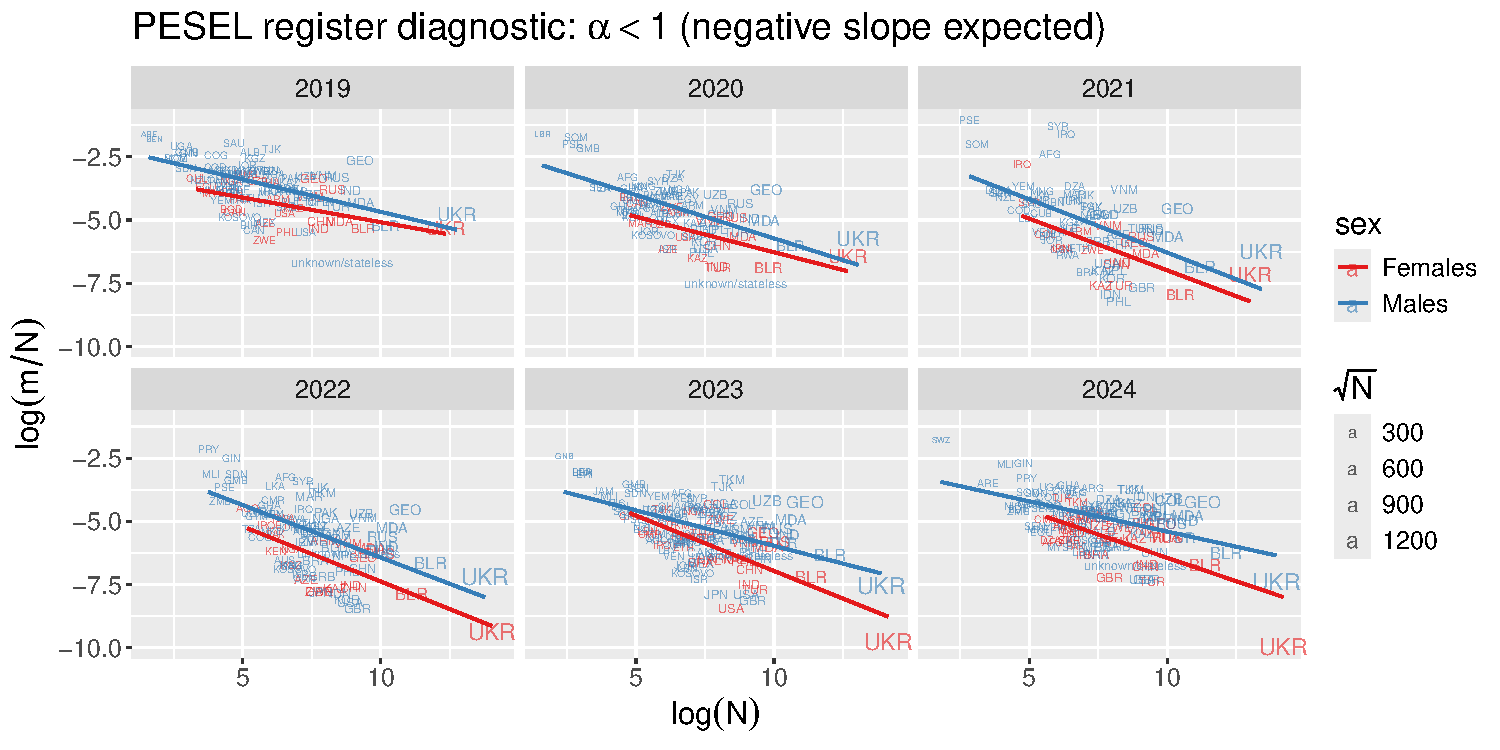
\includegraphics[width=0.9\textwidth]{figs-appen/figA-pesel-alpha.pdf}
    \caption{Diagnostic plot for community anchor ($\hat{\alpha}$): $\log(\text{Border/PESEL})$ vs $\log(\text{PESEL})$, by year and sex. Point size proportional to reference population. Slopes estimated from \eqref{eq-diagnostic-model} for each panel separately.}
    \label{fig-assumptions-population-pesel}
\end{figure}

\begin{figure}[ht!]
    \centering
    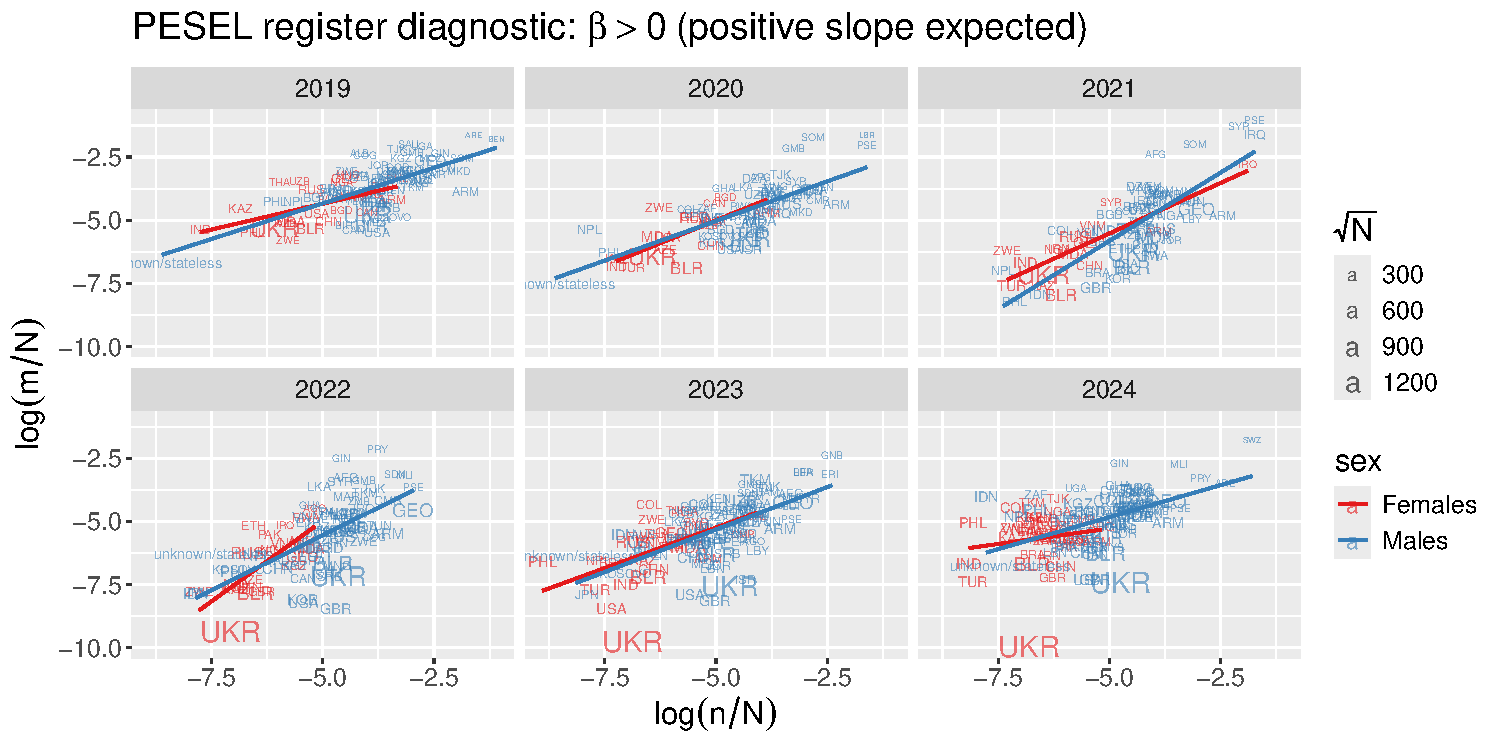
\includegraphics[width=0.9\textwidth]{figs-appen/figA-pesel-beta.pdf}
    \caption{Diagnostic plot for exposure elasticity ($\hat{\beta}$): $\log(\text{Border/PESEL})$ vs $\log(\text{Police/PESEL})$, by year and sex. Point size proportional to reference population. Slopes estimated from \eqref{eq-diagnostic-model} for each panel separately.}
    \label{fig-assumptions-population-pesel-police}
\end{figure}

\begin{figure}[ht!]
    \centering
    \includegraphics[width=0.9\textwidth]{figs-appen/figA-tax-alpha.pdf}
    \caption{Diagnostic plot for community anchor ($\hat{\alpha}$): $\log(\text{Border/Tax})$ vs $\log(\text{Tax})$, by year and sex. Point size proportional to reference population. Slopes estimated from \eqref{eq-diagnostic-model} for each panel separately.}
    \label{fig-assumptions-population-tax}
\end{figure}

\begin{figure}[ht!]
    \centering
    \includegraphics[width=0.9\textwidth]{figs-appen/figA-tax-beta.pdf}
    \caption{Diagnostic plot for exposure elasticity ($\hat{\beta}$): $\log(\text{Border/Tax})$ vs $\log(\text{Police/Tax})$, by year and sex. Point size proportional to reference population. Slopes estimated from \eqref{eq-diagnostic-model} for each panel separately.}
    \label{fig-assumptions-population-tax-police}
\end{figure}

\clearpage

\subsubsection{Year and continent (all
registers)}\label{year-and-continent-all-registers}

\begin{figure}[ht!]
    \centering
    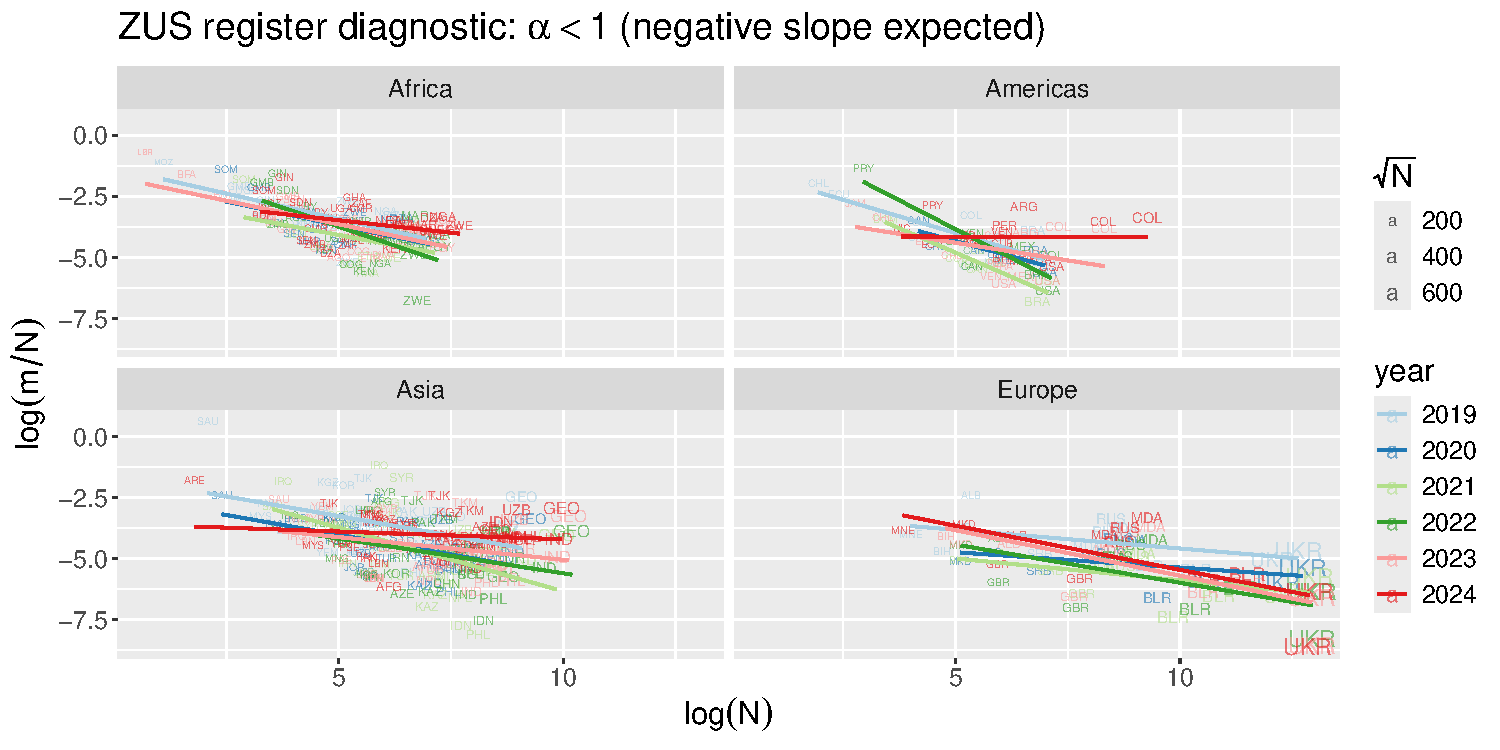
\includegraphics[width=0.9\textwidth]{figs-appen/figA-zus-alpha-continent.pdf}
    \caption{Diagnostic plot for community anchor ($\hat{\alpha}$): $\log(\text{Border/ZUS})$ vs $\log(\text{ZUS})$, by year and continent. Slopes estimated from \eqref{eq-diagnostic-model} for each panel separately. Oceania and stateless/unknown are suppressed due to small sample sizes.}
    \label{fig-assumptions-population-zus-continent}
\end{figure}

\begin{figure}[ht!]
    \centering
    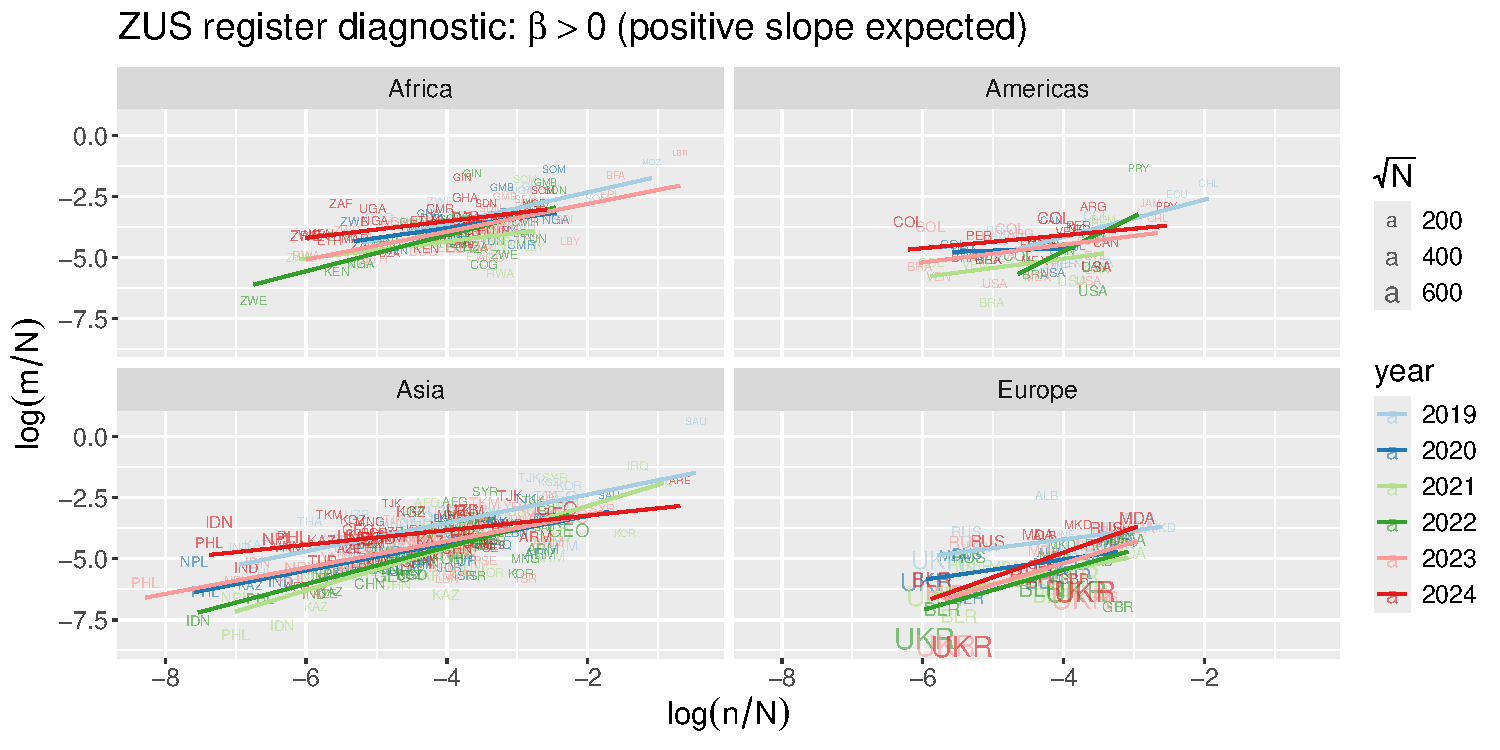
\includegraphics[width=0.9\textwidth]{figs-appen/figA-zus-beta-continent.pdf}
    \caption{Diagnostic plot for exposure elasticity ($\hat{\beta}$): $\log(\text{Border/ZUS})$ vs $\log(\text{Police/ZUS})$, by year and continent. Slopes estimated from \eqref{eq-diagnostic-model} for each panel separately. Grouping as in \autoref{fig-assumptions-population-zus-continent}.}
    \label{fig-assumptions-population-zus-police-continent}
\end{figure}

\begin{figure}[ht!]
    \centering
    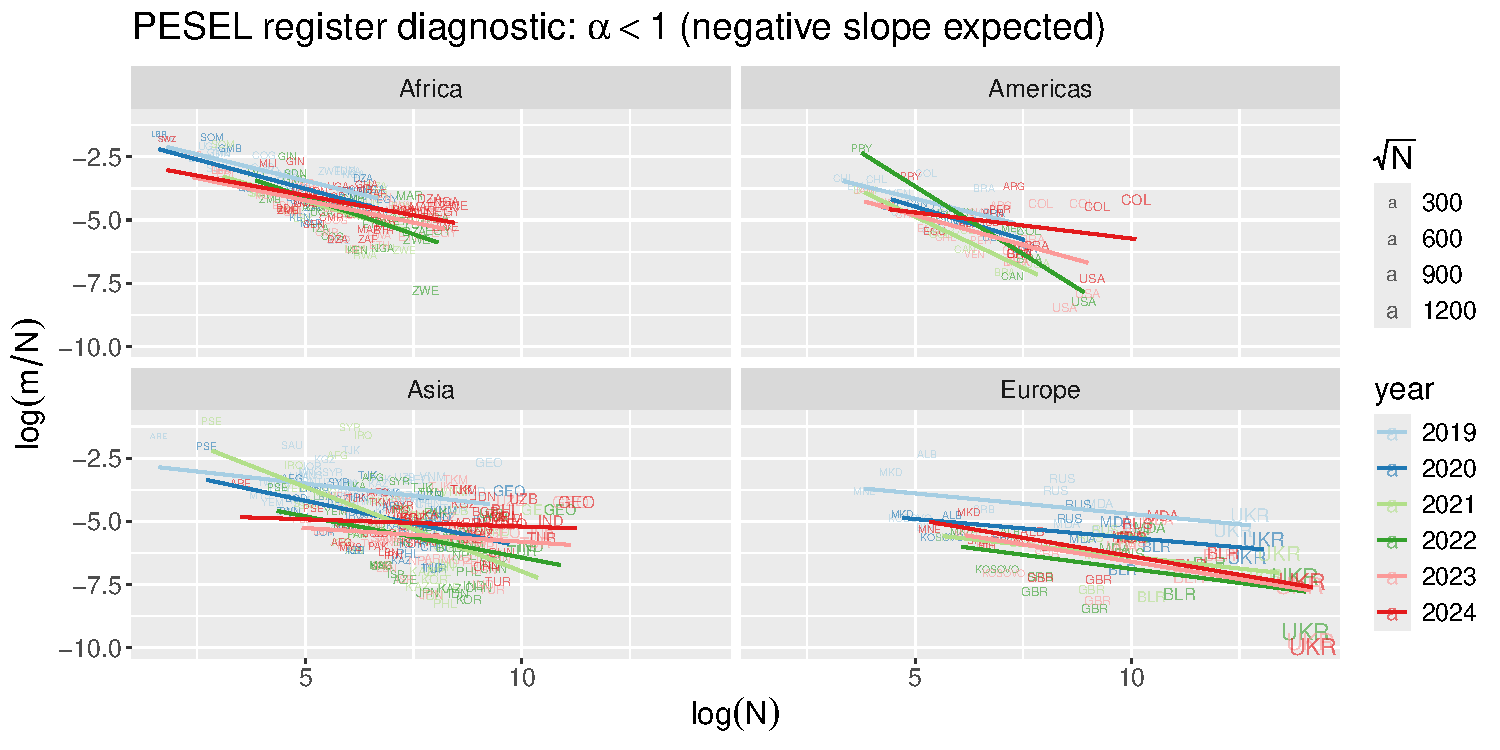
\includegraphics[width=0.9\textwidth]{figs-appen/figA-pesel-alpha-continent.pdf}
    \caption{Diagnostic plot for community anchor ($\hat{\alpha}$): $\log(\text{Border/PESEL})$ vs $\log(\text{PESEL})$, by year and continent. Slopes estimated from \eqref{eq-diagnostic-model} for each panel separately. Grouping as in \autoref{fig-assumptions-population-zus-continent}.}
    \label{fig-assumptions-population-pesel-continent}
\end{figure}

\begin{figure}[ht!]
    \centering
    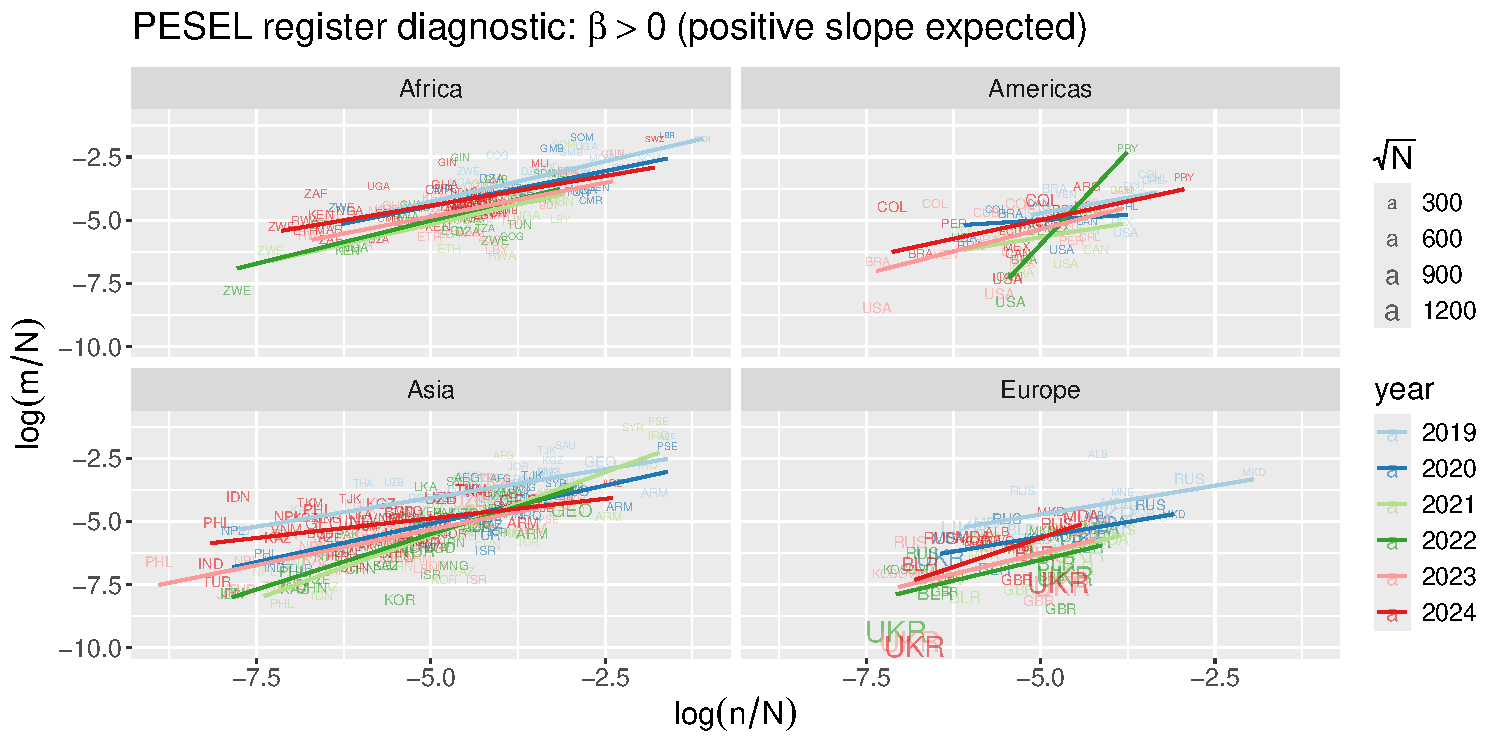
\includegraphics[width=0.9\textwidth]{figs-appen/figA-pesel-beta-continent.pdf}
    \caption{Diagnostic plot for exposure elasticity ($\hat{\beta}$): $\log(\text{Border/PESEL})$ vs $\log(\text{Police/PESEL})$, by year and continent. Slopes estimated from \eqref{eq-diagnostic-model} for each panel separately. Grouping as in \autoref{fig-assumptions-population-zus-continent}.}
    \label{fig-assumptions-population-pesel-police-continent}
\end{figure}

\begin{figure}[ht!]
    \centering
    \includegraphics[width=0.9\textwidth]{figs-appen/figA-tax-alpha-continent.pdf}
    \caption{Diagnostic plot for community anchor ($\hat{\alpha}$): $\log(\text{Border/Tax})$ vs $\log(\text{Tax})$, by year and continent. Slopes estimated from \eqref{eq-diagnostic-model} for each panel separately. Grouping as in \autoref{fig-assumptions-population-zus-continent}.}
    \label{fig-assumptions-population-tax-continent}
\end{figure}

\begin{figure}[ht!]
    \centering
    \includegraphics[width=0.9\textwidth]{figs-appen/figA-tax-beta-continent.pdf}
    \caption{Diagnostic plot for exposure elasticity ($\hat{\beta}$): $\log(\text{Border/Tax})$ vs $\log(\text{Police/Tax})$, by year and continent. Slopes estimated from \eqref{eq-diagnostic-model} for each panel separately. Grouping as in \autoref{fig-assumptions-population-zus-continent}.}
    \label{fig-assumptions-population-tax-police-continent}
\end{figure}

\clearpage

\section{Details about the models}\label{sec-appendix-covariate-comparison}

\subsection{AIC/BIC across eight specifications and three 
registers}\label{aicbic-across-eight-specifications-and-three-registers}

\begin{table}[ht!]
\caption{AIC and BIC for eight covariate specifications (S1--S8) across three registers and two estimation methods.} 
\fontsize{12.0pt}{14.0pt}\selectfont
\begin{tabular*}{\linewidth}{@{\extracolsep{\fill}}llrrrr}
\toprule
 &  & \multicolumn{2}{c}{{Poisson PMLE}} & \multicolumn{2}{c}{{NB-MLE}} \\ 
\cmidrule(lr){3-4} \cmidrule(lr){5-6}
Spec & Label & AIC & BIC & AIC & BIC \\ 
\midrule\addlinespace[2.5pt]
\multicolumn{6}{l}{ZUS} \\[2.5pt] 
\midrule\addlinespace[2.5pt]
S1 & Intercept only & 22,769.5 & 22,785.2 & 5,397.7 & 5,418.7 \\ 
S2 & Year & 16,870.9 & 16,938.9 & 5,283.0 & 5,356.3 \\ 
S3 & Year + sex & 16,447.0 & 16,520.2 & 5,274.5 & 5,353.0 \\ 
S4 & Year x UKR & 11,557.4 & 11,656.8 & 5,274.2 & 5,378.8 \\ 
S5 & Year x simplified & 14,321.7 & 14,421.1 & 5,283.7 & 5,388.4 \\ 
S6 & Year + continent & 12,859.7 & 12,953.9 & 5,245.8 & 5,345.2 \\ 
S7 & Year + sex + UKR & 14,231.3 & 14,309.8 & 5,272.8 & 5,356.5 \\ 
S8 & Year x UKR + sex & \textbf{11,535.6} & \textbf{11,640.2} & \textbf{5,265.2} & \textbf{5,375.0} \\ 
\midrule\addlinespace[2.5pt]
\multicolumn{6}{l}{Tax} \\[2.5pt] 
\midrule\addlinespace[2.5pt]
S1 & Intercept only & 24,688.2 & 24,704.7 & 5,833.1 & 5,855.2 \\ 
S2 & Year & 18,618.7 & 18,690.3 & 5,717.9 & 5,795.1 \\ 
S3 & Year + sex & 18,517.7 & 18,594.9 & 5,712.2 & 5,794.9 \\ 
S4 & Year x UKR & 13,509.4 & 13,614.2 & 5,715.8 & 5,826.1 \\ 
S5 & Year x simplified & 16,449.9 & 16,554.7 & 5,718.4 & 5,828.6 \\ 
S6 & Year + continent & 14,625.1 & 14,724.3 & 5,635.6 & 5,740.4 \\ 
S7 & Year + sex + UKR & 16,846.4 & 16,929.1 & 5,714.2 & 5,802.4 \\ 
S8 & Year x UKR + sex & \textbf{13,488.5} & \textbf{13,598.8} & \textbf{5,709.4} & \textbf{5,825.2} \\ 
\midrule\addlinespace[2.5pt]
\multicolumn{6}{l}{PESEL} \\[2.5pt] 
\midrule\addlinespace[2.5pt]
S1 & Intercept only & 24,604.3 & 24,620.9 & 5,820.0 & 5,842.1 \\ 
S2 & Year & 17,782.6 & 17,854.4 & 5,653.6 & 5,731.0 \\ 
S3 & Year + sex & 17,473.8 & 17,551.1 & 5,638.1 & 5,721.0 \\ 
S4 & Year x UKR & 12,561.5 & 12,666.5 & 5,645.5 & 5,756.1 \\ 
S5 & Year x simplified & 15,765.5 & 15,870.6 & 5,651.4 & 5,762.0 \\ 
S6 & Year + continent & 14,507.2 & 14,606.7 & 5,598.9 & 5,703.9 \\ 
S7 & Year + sex + UKR & 15,704.9 & 15,787.8 & 5,639.2 & 5,727.7 \\ 
S8 & Year x UKR + sex & \textbf{12,533.8} & \textbf{12,644.4} & \textbf{5,629.1} & \textbf{5,745.2} \\ 
\bottomrule
\end{tabular*}
\end{table}

Across all three registers, S8 ($\alpha$ varying by year $\times$ Ukrainian origin plus a sex effect) has the lowest Poisson PMLE AIC and BIC. The NB-MLE criteria differ little across specifications, with S8 within a few units of the best NB fit in every register, so we adopt S8 for both methods.
  

\clearpage

\subsection{Beta covariate selection}\label{sec-appendix-beta-selection}

The primary specification (S8) allows the exposure elasticity to vary by
year only. Here we examine whether enriching $\beta$ with sex and/or
Ukrainian origin improves the model. All specifications below share the
same S8 community anchor structure ($\alpha$ varying by year
$\times$ Ukrainian origin, plus a sex effect).


\begin{table}[ht!]
\caption{Effect of beta specification on AIC across three registers. S8 is the primary specification. All specifications share alpha = year x UKR + sex; k = number of parameters.} 
\fontsize{8.0pt}{10.0pt}\selectfont
\begin{tabular*}{\linewidth}{@{\extracolsep{\fill}}lclrrrl}
\toprule
Model & Spec & Covariates in beta & AIC & BIC & k & alpha > 1 \\ 
\midrule\addlinespace[2.5pt]
\multicolumn{7}{l}{ZUS} \\[2.5pt] 
\midrule\addlinespace[2.5pt]
NB-MLE & S8 & year & 5,265.2 & 5,375.0 & 21 & No \\ 
NB-MLE & S9 & year + sex & 5,266.3 & 5,381.3 & 22 & No \\ 
NB-MLE & S10 & year + UKR & 5,267.1 & 5,382.2 & 22 & No \\ 
NB-MLE & S11 & year + sex + UKR & 5,268.3 & 5,388.6 & 23 & No \\ 
Poisson PMLE & S8 & year & 11,535.6 & 11,640.2 & 20 & No \\ 
Poisson PMLE & S9 & year + sex & 11,527.7 & 11,637.5 & 21 & No \\ 
Poisson PMLE & S10 & year + UKR & 11,497.4 & 11,607.2 & 21 & No \\ 
Poisson PMLE & S11 & year + sex + UKR & 11,402.3 & 11,517.4 & 22 & No \\ 
\midrule\addlinespace[2.5pt]
\multicolumn{7}{l}{Tax} \\[2.5pt] 
\midrule\addlinespace[2.5pt]
NB-MLE & S8 & year & 5,709.4 & 5,825.2 & 21 & No \\ 
NB-MLE & S9 & year + sex & 5,711.4 & 5,832.7 & 22 & No \\ 
NB-MLE & S10 & year + UKR & 5,711.4 & 5,832.7 & 22 & No \\ 
NB-MLE & S11 & year + sex + UKR & 5,713.4 & 5,840.2 & 23 & No \\ 
Poisson PMLE & S8 & year & 13,488.5 & 13,598.8 & 20 & No \\ 
Poisson PMLE & S9 & year + sex & 13,471.5 & 13,587.3 & 21 & No \\ 
Poisson PMLE & S10 & year + UKR & 13,352.4 & 13,468.2 & 21 & No \\ 
Poisson PMLE & S11 & year + sex + UKR & 13,118.0 & 13,239.4 & 22 & No \\ 
\midrule\addlinespace[2.5pt]
\multicolumn{7}{l}{PESEL} \\[2.5pt] 
\midrule\addlinespace[2.5pt]
NB-MLE & S8 & year & 5,629.1 & 5,745.2 & 21 & No \\ 
NB-MLE & S9 & year + sex & 5,628.5 & 5,750.1 & 22 & No \\ 
NB-MLE & S10 & year + UKR & 5,631.0 & 5,752.6 & 22 & No \\ 
NB-MLE & S11 & year + sex + UKR & 5,630.4 & 5,757.6 & 23 & No \\ 
Poisson PMLE & S8 & year & 12,533.8 & 12,644.4 & 20 & No \\ 
Poisson PMLE & S9 & year + sex & 12,532.0 & 12,648.1 & 21 & No \\ 
Poisson PMLE & S10 & year + UKR & 12,368.3 & 12,484.4 & 21 & No \\ 
Poisson PMLE & S11 & year + sex + UKR & 12,295.7 & 12,417.3 & 22 & No \\ 
\bottomrule
\end{tabular*}
\end{table}




Extending $\beta$ with sex and Ukrainian origin (S9–S11) lowers the Poisson AIC in every register, but leaves the NB AIC essentially unchanged (and marginally higher). Because the additional $\beta$ terms improve only the Poisson fit while S8 already minimises or nearly minimises the NB AIC, we keep $\beta$ varying by year only, giving a parsimonious specification that is comparable across both methods and all three registers.

\clearpage

\subsection{UKR vs non-UKR alpha trajectories across
specifications}\label{ukr-vs-non-ukr-alpha-trajectories-across-specifications}

\begin{figure}[ht!]
    \centering
    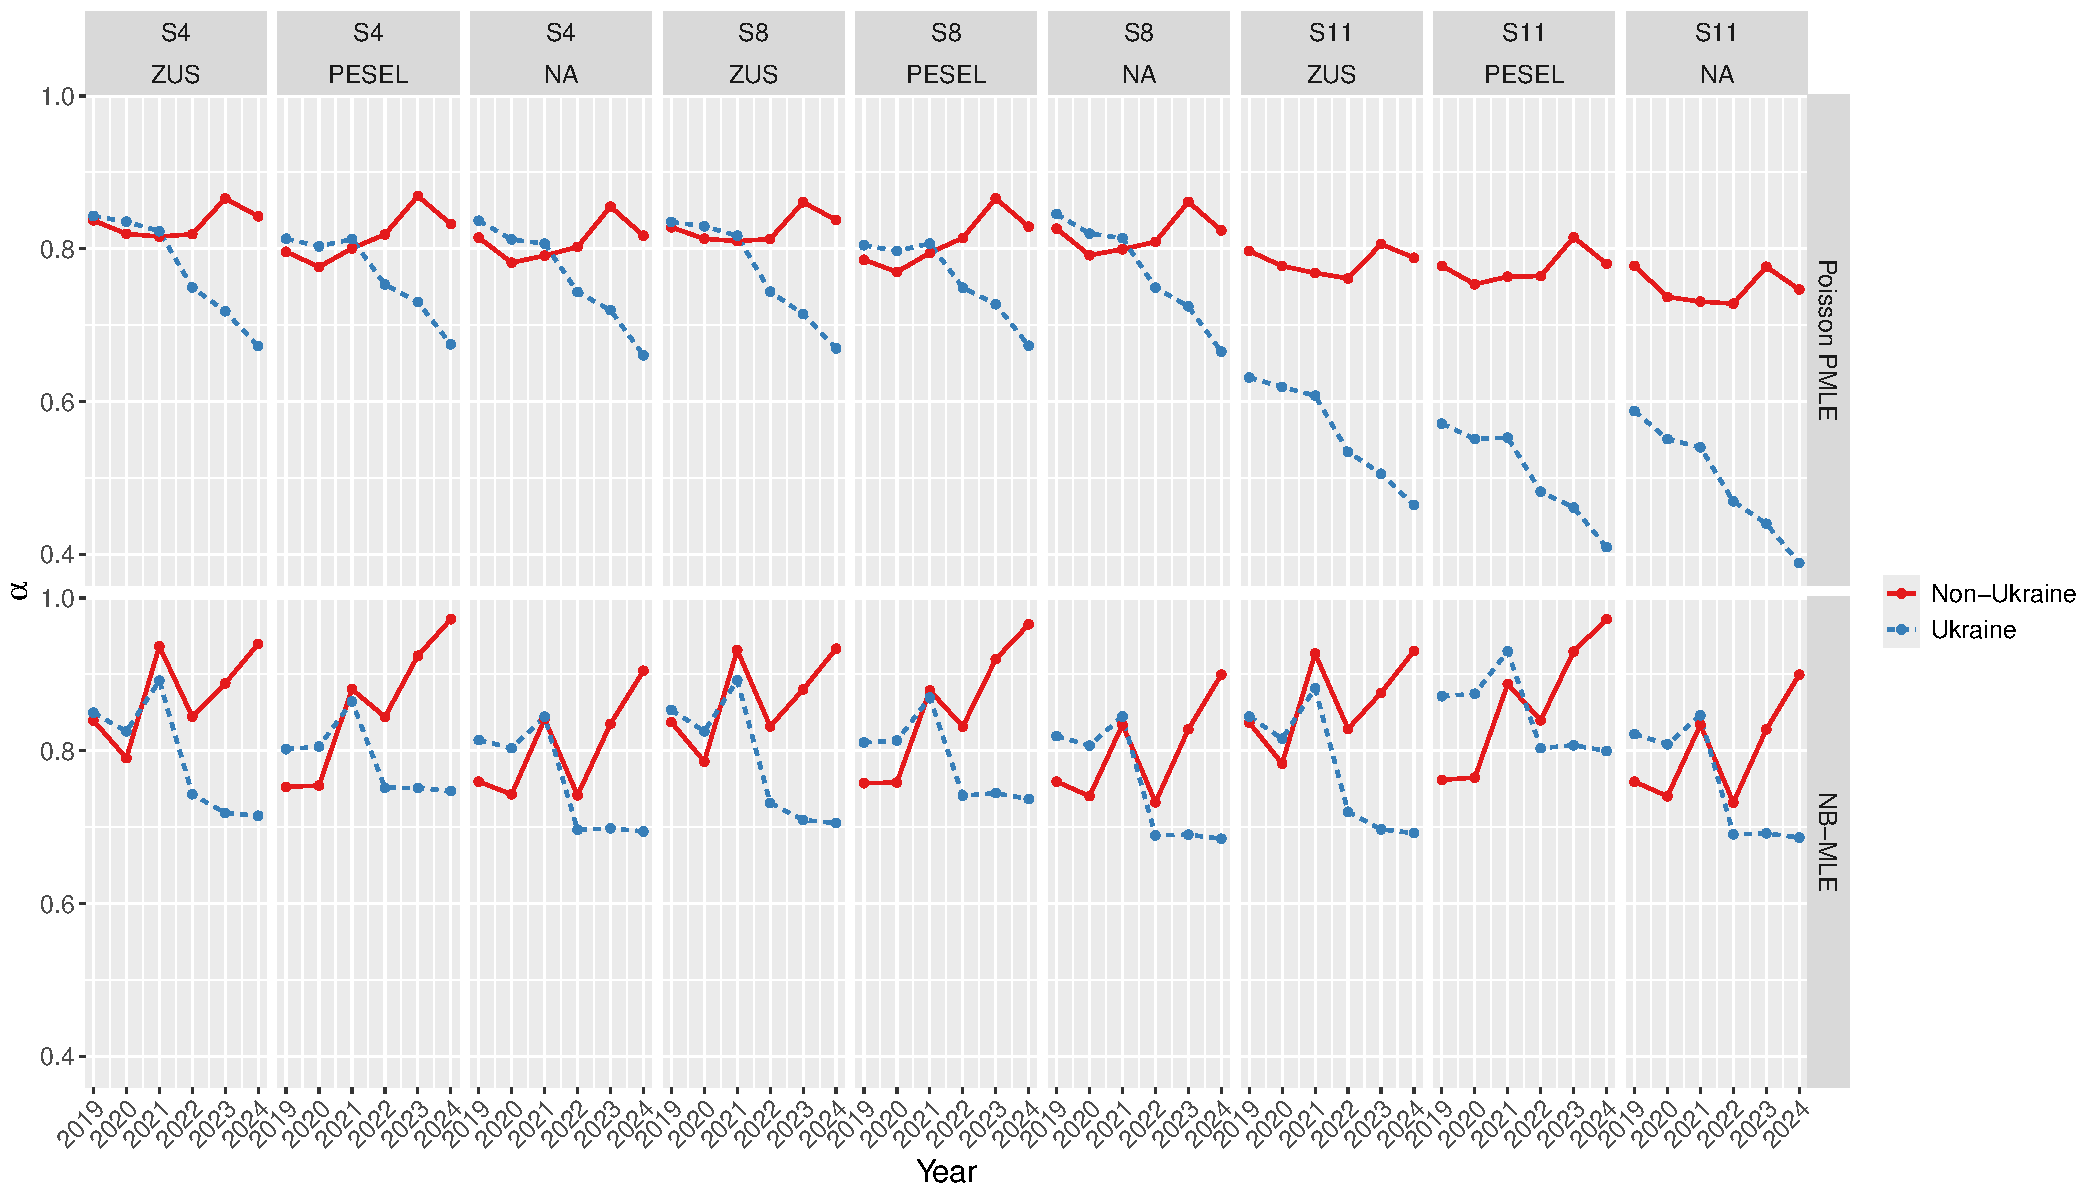
\includegraphics[width=0.9\textwidth]{figs-appen/figA-alpha-ukr-appendix.pdf}
    \caption{\label{fig-alpha-ukr-appendix}UKR vs non-UKR alpha trajectories
across three specifications (S4, S8, S11) and three registers. Under S8
and S11, the sex covariate shifts both trajectories. Under S11, the
extended beta coefficients change the jointly estimated alpha values. The Poisson
trajectories are more stable across specifications.}
\end{figure}

\clearpage

\subsection{Coefficient estimates}\label{sec-appendix-coefficients}

Table~\ref{tbl-coefficients-appendix} presents the S8 coefficient
estimates under Poisson PML and unconstrained NB. Both columns are on
the original $\alpha$ and $\beta$ scale and are directly comparable.
The constrained NB is also fit (with $\alpha \in (0,1)$ enforced via a
logit link) but its coefficients are on the link scale and therefore not
magnitude-comparable to the other two; we report the resulting
$\alpha$ values per cell --- already back-transformed --- in
Table~\ref{tbl-alpha-cells}, alongside the Poisson and NB values for
direct comparison.

\begin{table}[ht!]
\caption{\label{tbl-coefficients-appendix}S8 coefficient estimates under Poisson PML and unconstrained NB. Cluster fractional-weighted bootstrap medians with 95\% percentile confidence intervals in parentheses (R = 999, clustered by country). ZUS reference population. Both models unconstrained.} 
\fontsize{8.0pt}{10.0pt}\selectfont
\begin{tabular*}{\linewidth}{@{\extracolsep{\fill}}lrr}
\toprule
 & Poisson & NB \\ 
\midrule\addlinespace[2.5pt]
\multicolumn{3}{l}{Community anchor ($\hat{\alpha}$)} \\[2.5pt] 
\midrule\addlinespace[2.5pt]
Intercept (2019, female, non-UKR) & 0.822 (0.627, 0.967) & 0.813 (0.708, 0.900) \\ 
Year 2020 & -0.012 (-0.061, 0.036) & -0.049 (-0.159, 0.051) \\ 
Year 2021 & -0.010 (-0.110, 0.145) & 0.097 (-0.012, 0.220) \\ 
Year 2022 & -0.012 (-0.133, 0.148) & 0.012 (-0.178, 0.150) \\ 
Year 2023 & 0.037 (-0.077, 0.190) & 0.044 (-0.049, 0.148) \\ 
Year 2024 & 0.014 (-0.073, 0.168) & 0.097 (0.012, 0.190) \\ 
Ukrainian origin & 0.008 (-0.059, 0.094) & 0.018 (-0.031, 0.075) \\ 
Male & 0.018 (-0.010, 0.043) & 0.046 (0.015, 0.080) \\ 
Year 2020 $\times$ Ukrainian & 0.007 (-0.016, 0.026) & 0.023 (-0.020, 0.070) \\ 
Year 2021 $\times$ Ukrainian & -0.005 (-0.077, 0.040) & -0.056 (-0.120, -0.002) \\ 
Year 2022 $\times$ Ukrainian & -0.082 (-0.152, -0.030) & -0.122 (-0.196, -0.040) \\ 
Year 2023 $\times$ Ukrainian & -0.158 (-0.224, -0.112) & -0.187 (-0.243, -0.143) \\ 
Year 2024 $\times$ Ukrainian & -0.177 (-0.242, -0.145) & -0.244 (-0.297, -0.201) \\ 
\midrule\addlinespace[2.5pt]
\multicolumn{3}{l}{Exposure elasticity ($\hat{\beta}$)} \\[2.5pt] 
\midrule\addlinespace[2.5pt]
Intercept (2019) & 0.730 (0.360, 1.220) & 0.887 (0.653, 1.183) \\ 
Year 2020 & 0.166 (0.057, 0.307) & 0.132 (-0.097, 0.368) \\ 
Year 2021 & 0.246 (0.023, 0.570) & 0.516 (0.290, 0.805) \\ 
Year 2022 & 0.208 (-0.064, 0.539) & 0.261 (-0.150, 0.582) \\ 
Year 2023 & 0.193 (-0.072, 0.500) & 0.240 (0.035, 0.493) \\ 
Year 2024 & -0.009 (-0.219, 0.290) & 0.180 (0.002, 0.368) \\ 
\midrule\addlinespace[2.5pt]
\multicolumn{3}{l}{Fit statistics} \\[2.5pt] 
\midrule\addlinespace[2.5pt]
Num.Obs. & 1,382 & 1,382 \\ 
AIC & 11535.6 & 5265.2 \\ 
BIC & 11640.2 & 5375.0 \\ 
Log.Lik. & -5747.784 & -2611.580 \\ 
\bottomrule
\end{tabular*}
\end{table}






Table~\ref{tbl-alpha-cells} shows the actual $\alpha$ values per cell
(year $\times$ Ukrainian origin $\times$ sex) under all three
specifications: Poisson PML, unconstrained NB, and constrained NB
(back-transformed via $\text{logit}^{-1}$). Reporting all three on a
common scale makes the constrained-vs-unconstrained NB comparison
transparent: the constraint barely binds on Polish data (the
unconstrained NB already produces $\alpha < 1$ in every cell). The
unconstrained NB nonetheless pushes $\alpha$ close to 1 for
non-Ukrainian males in recent years (0.96 in 2024), which is the primary
driver of the higher NB population size estimates documented in the main
text.


\begin{table}[ht!]
\caption{\label{tbl-alpha-cells}$\alpha$ values per (year, Ukrainian origin, sex) cell under three specifications. Constrained NB back-transformed via logit-inverse.} 
\fontsize{8.0pt}{10.0pt}\selectfont
\begin{tabular*}{\linewidth}{@{\extracolsep{\fill}}rllrrr}
\toprule
Year & Origin & Sex & NB & NB (constrained) & Poisson \\ 
\midrule\addlinespace[2.5pt]
2019 & UKR & Females & 0.8311 & 0.8391 & 0.8297 \\ 
2019 & UKR & Males & 0.8758 & 0.8896 & 0.8406 \\ 
2019 & Non-UKR & Females & 0.8137 & 0.8416 & 0.8222 \\ 
2019 & Non-UKR & Males & 0.8583 & 0.8914 & 0.8331 \\ 
2020 & UKR & Females & 0.8032 & 0.8095 & 0.8238 \\ 
2020 & UKR & Males & 0.8478 & 0.8679 & 0.8348 \\ 
2020 & Non-UKR & Females & 0.7618 & 0.7575 & 0.8072 \\ 
2020 & Non-UKR & Males & 0.8065 & 0.8283 & 0.8182 \\ 
2021 & UKR & Females & 0.8699 & 0.8597 & 0.8117 \\ 
2021 & UKR & Males & 0.9146 & 0.9045 & 0.8226 \\ 
2021 & Non-UKR & Females & 0.9075 & 0.8840 & 0.8040 \\ 
2021 & Non-UKR & Males & 0.9522 & 0.9217 & 0.8150 \\ 
2022 & UKR & Females & 0.7095 & 0.6669 & 0.7383 \\ 
2022 & UKR & Males & 0.7542 & 0.7557 & 0.7493 \\ 
2022 & Non-UKR & Females & 0.8090 & 0.7638 & 0.8072 \\ 
2022 & Non-UKR & Males & 0.8537 & 0.8333 & 0.8182 \\ 
2023 & UKR & Females & 0.6871 & 0.6626 & 0.7091 \\ 
2023 & UKR & Males & 0.7318 & 0.7522 & 0.7201 \\ 
2023 & Non-UKR & Females & 0.8576 & 0.8639 & 0.8554 \\ 
2023 & Non-UKR & Males & 0.9023 & 0.9075 & 0.8663 \\ 
2024 & UKR & Females & 0.6829 & 0.6596 & 0.6642 \\ 
2024 & UKR & Males & 0.7276 & 0.7496 & 0.6751 \\ 
2024 & Non-UKR & Females & 0.9104 & 0.9430 & 0.8320 \\ 
2024 & Non-UKR & Males & 0.9551 & 0.9623 & 0.8429 \\ 
\bottomrule
\end{tabular*}
\end{table}




\clearpage

\subsection{Estimates across reference registers}\label{sec-appendix-multi-register}

  Figure~\ref{fig-multi-register-size} reports the estimated unauthorised
  population (in thousands) and Figure~\ref{fig-multi-register} the same
  estimates as a share of the reference population ($\hat\xi / N$), in both
  cases by reference register (PESEL, Tax, ZUS), origin (Ukrainian vs
  non-Ukrainian), and estimation method (Poisson PMLE, NB-MLE). In recent years
  the Ukrainian share is much smaller than the non-Ukrainian share, because the
  2022 Temporary Protection Directive expanded the Ukrainian reference population
  $N$ without a matching increase in the unauthorised count $m$.
  
  \begin{figure}[ht!]
      \centering
      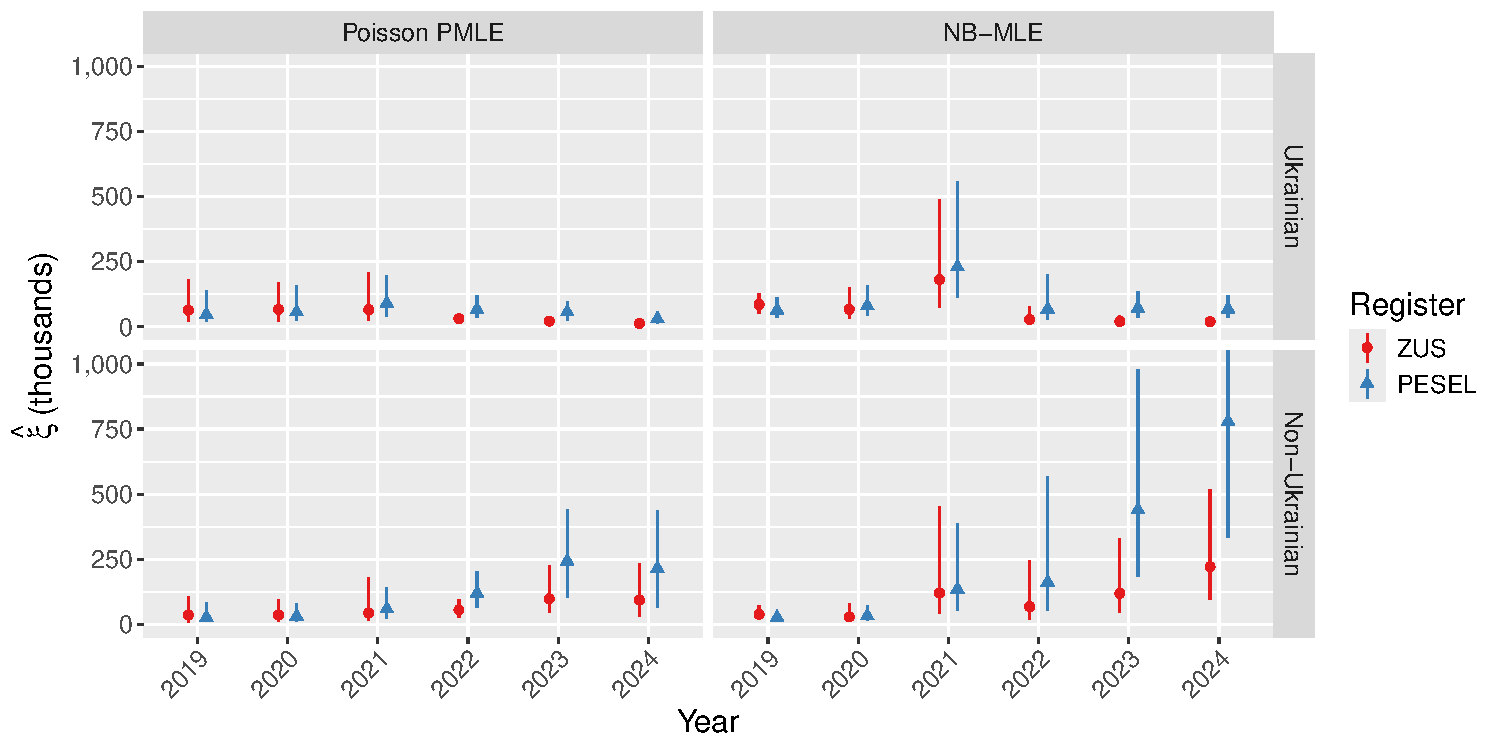
\includegraphics[width=0.9\textwidth]{figs-appen/figA-popsize-register.pdf}
      \caption{\label{fig-multi-register-size}Estimated unauthorised population
  (in thousands) by reference register (PESEL, Tax, ZUS), origin (Ukrainian vs
  non-Ukrainian), and estimation method (Poisson PMLE, NB-MLE). Points are
  cluster fractional-weighted bootstrap medians with 95\% percentile confidence
  intervals ($R = 199$, clustered by country); values are truncated at one
  million.}
  \end{figure} 

  \begin{figure}[ht!]
      \centering
      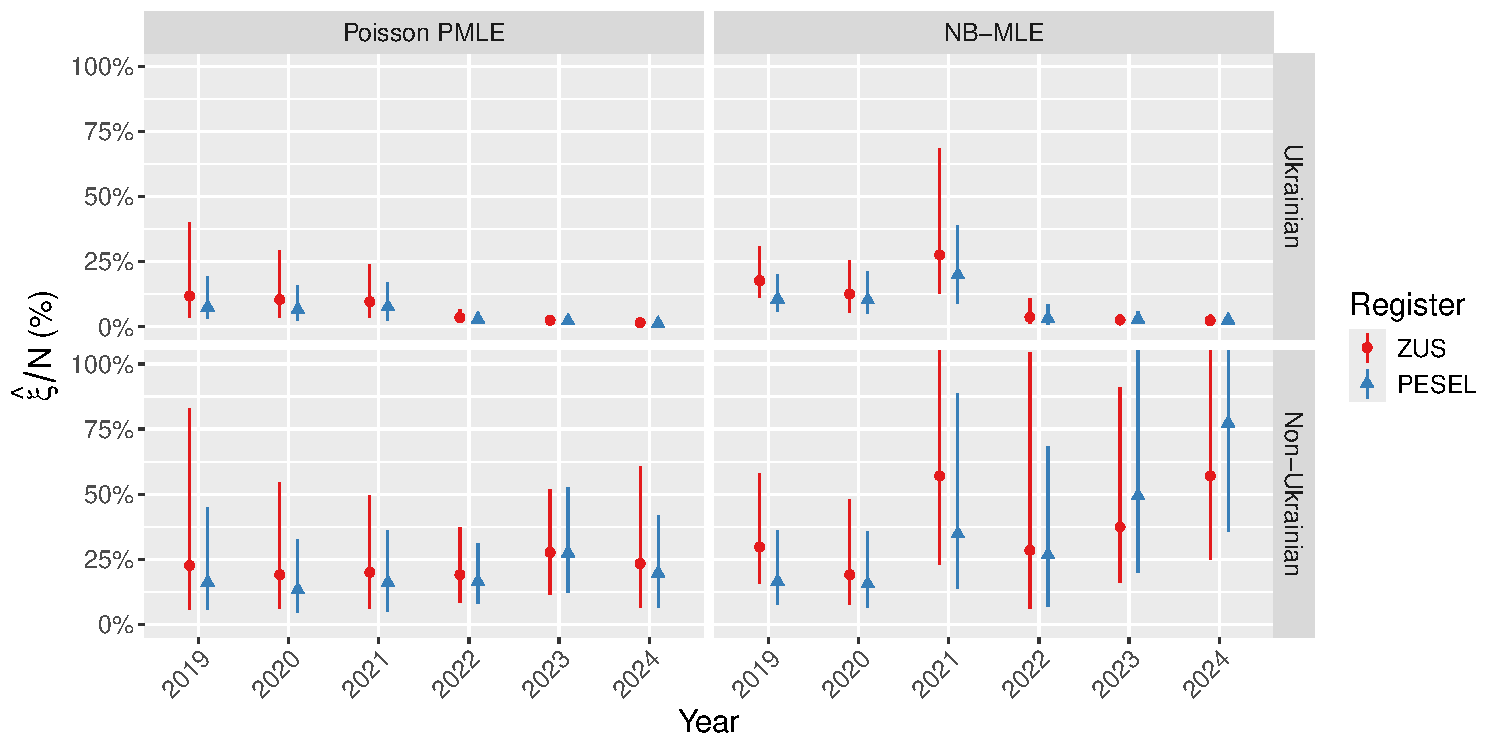
\includegraphics[width=0.9\textwidth]{figs-appen/figA-popsize-share.pdf}
      \caption{\label{fig-multi-register}Estimated unauthorised population as a
  share of the reference population ($\hat\xi / N$), by register, origin, and
  estimation method. Points are cluster fractional-weighted bootstrap medians
  with 95\% percentile confidence intervals ($R = 199$, clustered by country);
  shares are truncated at 100\%.}
  \end{figure}
  
  Under Poisson, the shares are similar across registers. The Ukrainian share
  falls from about 8--13\% in 2019 to about 1\% in 2024, following the post-2022
  growth of the denominator. The non-Ukrainian share is about 14--27\% through
  2022 and 17--30\% afterwards, with confidence intervals that overlap across the
  three registers.
  
  Under NB, several non-Ukrainian point estimates exceed 50\% of the reference
  population (for example PESEL at 79\% and ZUS at 61\% in 2024), and some upper
  confidence bounds exceed 100\% and are truncated in the figure. These values
  follow from the $\gamma$--$\theta$ confounding discussed in
  Section~\ref{sec-simulation}, which inflates $\hat\alpha$ and hence
  $\hat\xi$ under the NB variance function. We use Poisson as the primary
  estimator and NB as a sensitivity bound.

\clearpage
\section{Estimates across different auxiliary counts ($n$)}\label{sec-appendix-auxiliary-counts}

S8 uses the police count as the auxiliary detection variable $n$. We refit S8 against the ZUS reference, replacing $n$ with each of three counts: all adult police records (police total), the subset whose subject held a PESEL number (police PESEL ID), and prison records. The three datasets share the same $m$, $N$ and cells, so any change in $\hat\xi$ comes from the auxiliary source alone. Table~\ref{tbl-nsource-aux} reports the two features that set how informative each $n$ is. All three correlate positively with $m$, but the rank correlation falls from $0.73$ (police total) to $0.62$ (prison). The detection slope $\beta$ is identified only from cells with $m_{it}n_{it}>0$, and the zero share rises from $30\%/69\%$ (males/females) for police total to $59\%/91\%$ for prison. With $91\%$ of female prison cells empty, the female slope rests on under a tenth of the data, the small-counts regime that destabilises NB-MLE (Section~\ref{sec-simulation}).


Poisson PMLE, our primary estimator, is insensitive to this choice. Its yearly trajectory is stable across the three counts, with summed totals of $503$--$591$ thousand (Table~\ref{tbl-nsource-fit}) and broadly overlapping $80\%$ and $95\%$ percentile intervals (Figure~\ref{fig-nsource-year}), and the same agreement holds by Ukrainian origin (Figure~\ref{fig-nsource-ukr}). NB-MLE attains lower AIC and BIC, but, as in the main text, this reflects its accommodation of over-dispersion rather than a better mean structure: under all three counts it reproduces the implausible 2021 and 2024 spikes, so we report it only as a sensitivity bound. The one visible exception is the PESEL-ID estimate for 2021, which drops across all groups (Figures~\ref{fig-nsource-year}--\ref{fig-nsource-sex}): its yearly elasticity $\beta_{2021}$ flattens while the PESEL count rises relative to apprehensions, inflating the fitted detection rate and shrinking $\hat\xi = m/\rho$, and because $\beta_t$ is common across communities the dip is uniform over origin and sex; it rests on the year's fewest identifying cells ($m_{it}n_{it}>0$), so we read it as a small-counts artefact rather than a real decline. Away from those 2021 and 2024 spikes, the NB-MLE medians lie within the Poisson $95\%$ intervals, so the reported estimates are robust in this respect. The sex split (Figure~\ref{fig-nsource-sex}) is the stress test: female estimates are several times smaller and carry the widest relative intervals, the prison-female series is the least stable, and males drive the totals. The S8 estimates by Poisson PMLE thus hold across all three detection counts; prison, the weakest and sparsest proxy, is a corroborating check only.
  
 \begin{table}[H]
  \centering
  \caption{\label{tbl-nsource-aux}Auxiliary detection counts used in the S8 sensitivity check: Pearson and Spearman correlation with the apprehension count $m$ across
  community--year--sex cells, and the share of cells with a zero auxiliary count by sex.}
  \begin{tabular}{lrrrr} \toprule
  Auxiliary count ($n$) & Pearson $r(m,n)$ & Spearman $\rho(m,n)$ & Zeros, Females (\%) & Zeros, Males (\%) \\ \midrule
  Police (total) & 0.71 & 0.73 & 69 & 30 \\
  Police (PESEL ID) & 0.53 & 0.71 & 79 & 37 \\
  Prison & 0.66 & 0.62 & 91 & 59 \\
  \bottomrule
  \end{tabular}
  \end{table}

  
  \begin{table}[H]
  \centering
  \caption{\label{tbl-nsource-fit}Model fit and estimated population size under S8 with three auxiliary detection counts. AIC and BIC for Poisson PMLE and NB-MLE; $\hat\xi$ is the sum of the yearly point estimates (in thousands). Lower NB-MLE AIC/BIC reflects over-dispersion accommodation and is not grounds for preferring it
  (Section~\ref{sec-cov-selection}).}
  \begin{tabular}{lrrrr|rr} \toprule
  & \multicolumn{2}{c}{Poisson PMLE} & \multicolumn{2}{c|}{NB-MLE} & \multicolumn{2}{c}{$\hat\xi$ (000s)} \\
  Auxiliary count ($n$) & AIC & BIC & AIC & BIC & Po & NB \\ \midrule
  Police (total) & 11,536 & 11,640 & 5,265 & 5,375 & 591 & 997 \\
  Police (PESEL ID) & 13,214 & 13,319 & 5,438 & 5,548 & 503 & 777 \\
  Prison & 13,510 & 13,614 & 5,355 & 5,465 & 583 & 894 \\
  \bottomrule
  \end{tabular}
  \end{table}

  \begin{figure}[ht!]
      \centering
      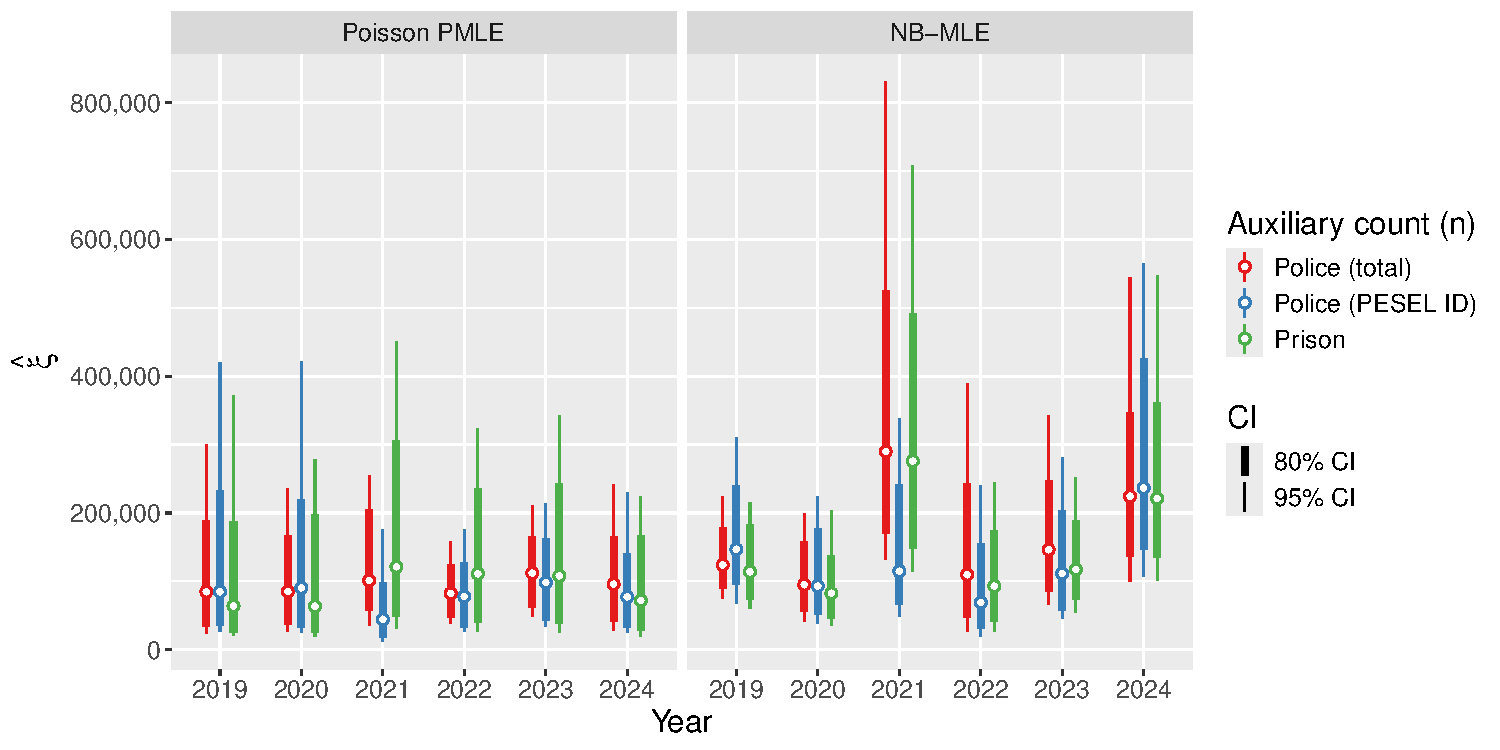
\includegraphics[width=\textwidth]{figs-appen/figA-nsource-year.pdf}
      \caption{\label{fig-nsource-year}Estimated population $\hat\xi$ by year under S8, refitted
  with three auxiliary detection counts $n$, by estimation method. The counts are: police total
  (all adult police records in criminal or registration proceedings), police PESEL ID (the
  subset whose subject held a PESEL number), and prison (prison records). Points are cluster
  fractional-weighted bootstrap medians; thick bars give $80\%$ and thin bars $95\%$ percentile
  confidence intervals (199 replicates, clustered by country).}
  \end{figure}

  \begin{figure}[ht!]
      \centering
      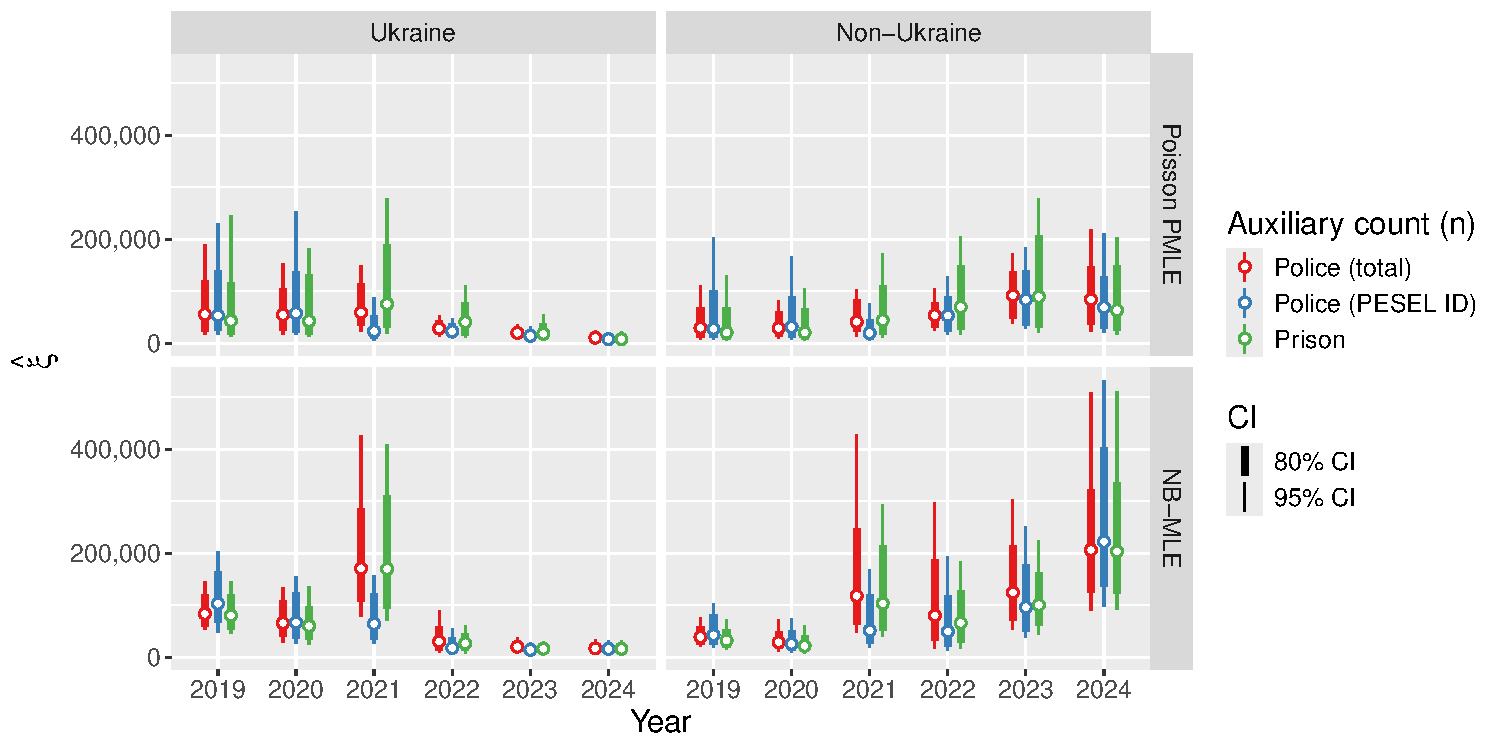
\includegraphics[width=\textwidth]{figs-appen/figA-nsource-ukr.pdf}
      \caption{\label{fig-nsource-ukr}As Figure~\ref{fig-nsource-year}, by Ukrainian versus
  non-Ukrainian origin.}
  \end{figure}

  \begin{figure}[ht!]
      \centering
      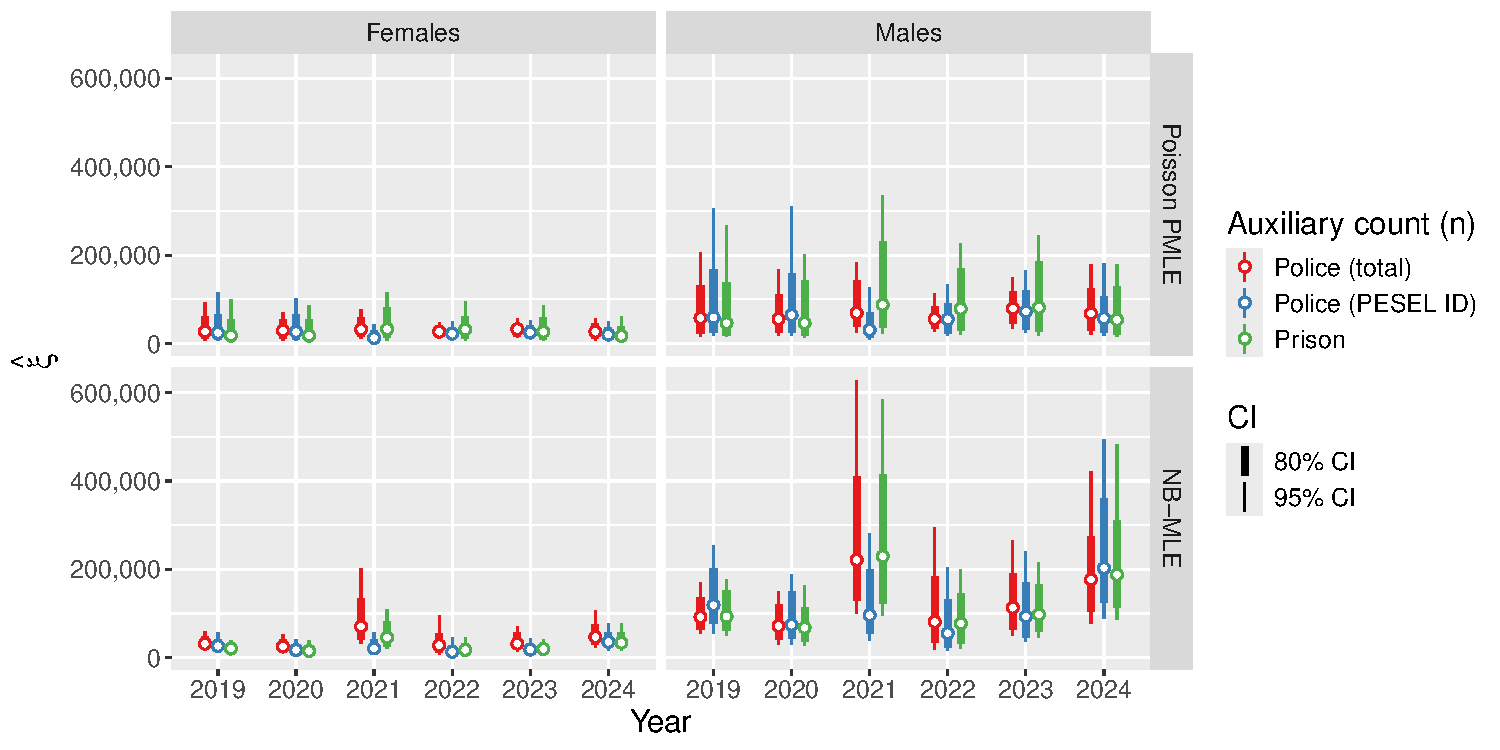
\includegraphics[width=\textwidth]{figs-appen/figA-nsource-sex.pdf}
      \caption{\label{fig-nsource-sex}As Figure~\ref{fig-nsource-year}, by sex. The prison count
  is zero in $91\%$ of female cells, which inflates the female intervals.}
  \end{figure}
  
  
\clearpage
\section{Model diagnostics for S8 specification}\label{sec-appendix-diagnostics}

\subsection{Country-level leave-one-out sensitivity for the S8
specification}\label{country-level-leave-one-out-sensitivity-for-the-s8-specification}

Figure~\ref{fig-loo-s8} shows leave-one-out sensitivity by country of
origin under S8: each bar is the change in $\hat\xi$ when that country
is dropped. Ukraine is excluded, because dropping it removes the entire
UKR stratum and leaves the year-by-UKR interaction unidentifiable. Under
Poisson, leverage is concentrated in Belarus ($+64\%$) and Georgia
($-49\%$), with no other country above about $6\%$. Under NB the
effects are smaller and more spread out, the largest being the
unknown/stateless group ($+13\%$), Vietnam ($-9\%$), and Georgia
($-8\%$). The main-text cluster fractional-weighted bootstrap clusters
by country of origin precisely to absorb this dependence.

\begin{figure}[ht!]
    \centering
    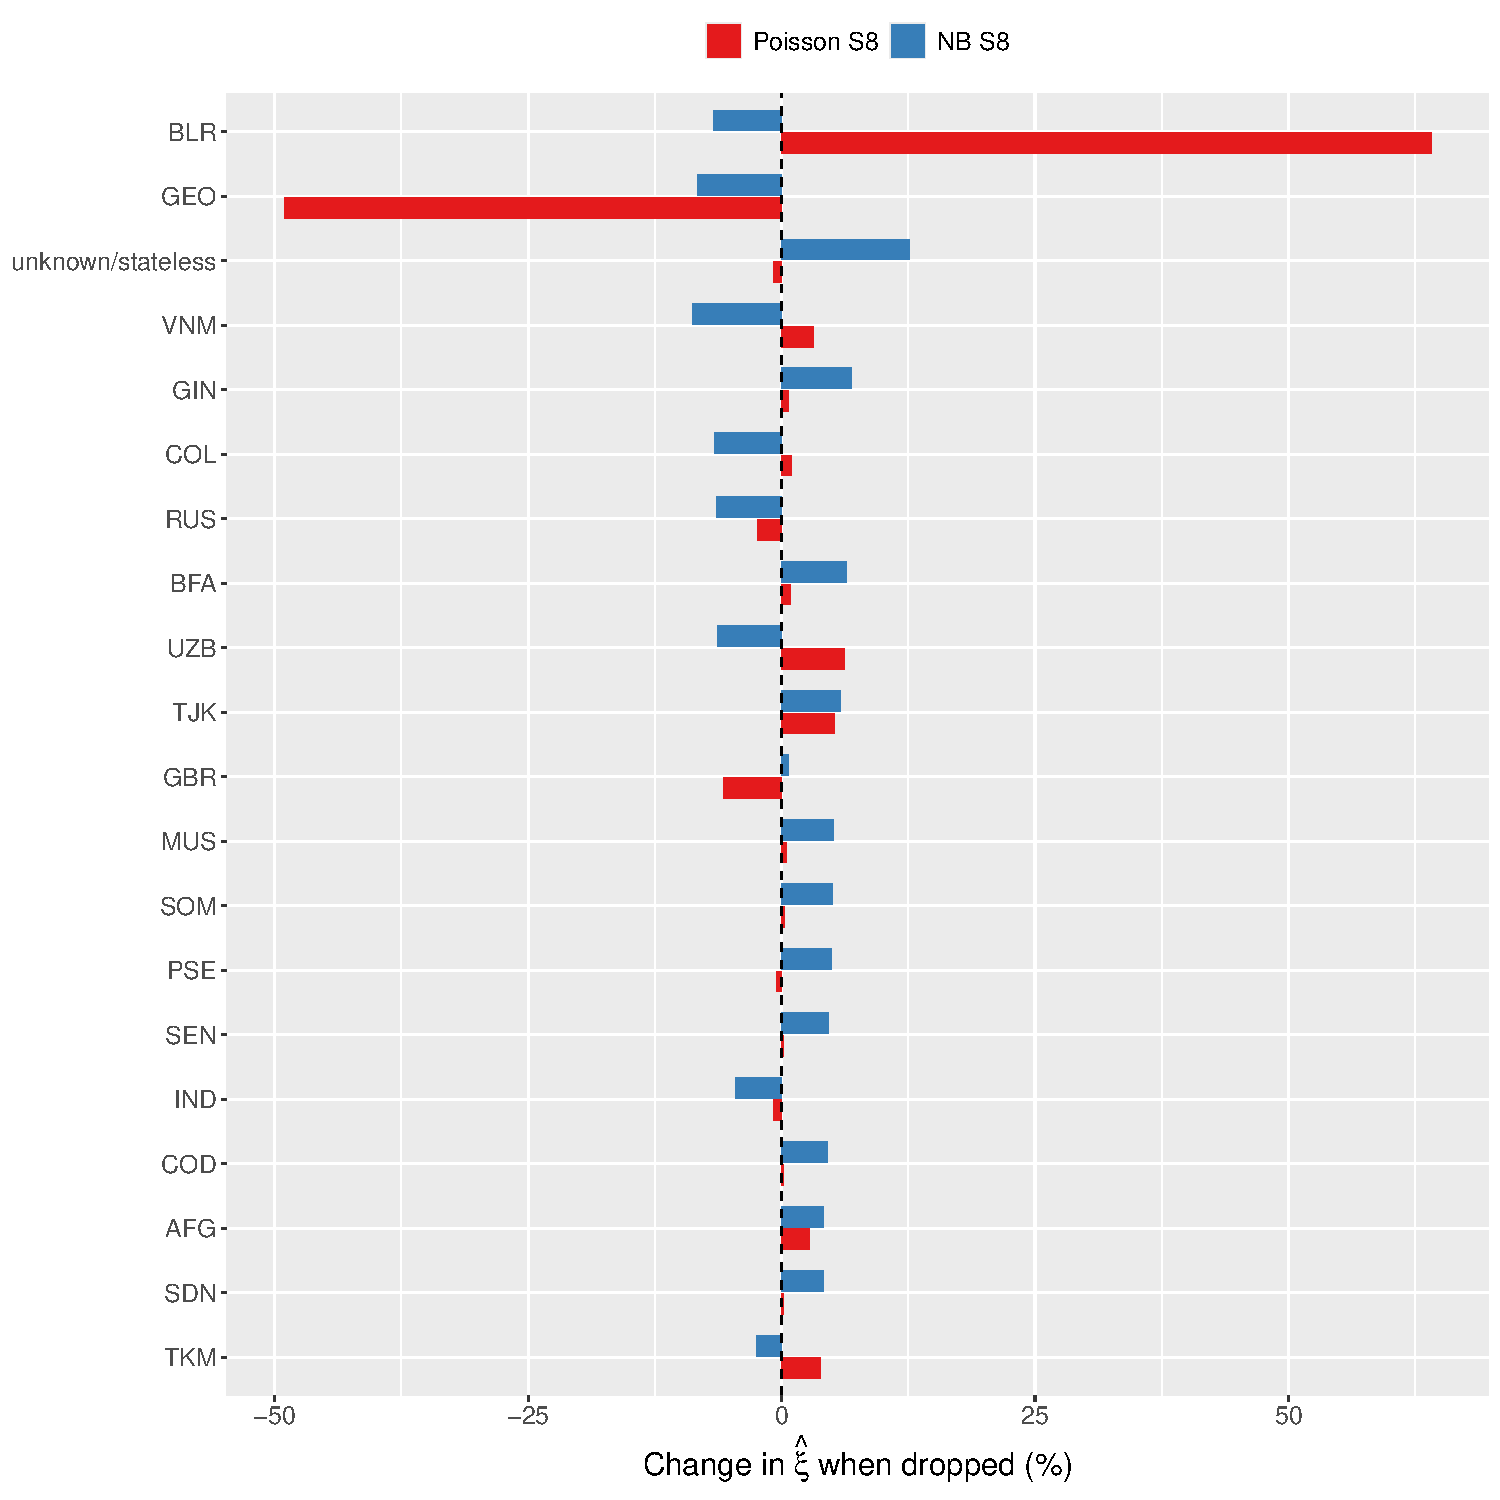
\includegraphics[width=0.9\textwidth]{figs-appen/figA-loo-s8.pdf}
    \caption{\label{fig-loo-s8}Leave-one-out sensitivity by country of
origin under S8: change in $\hat\xi$ when each country is dropped, top
20 shown (Ukraine excluded). Poisson is dominated by a few origins;
NB influence is smaller and more evenly spread, reflecting its quadratic
variance function.}
\end{figure}

Because Ukraine is the only country in the UKR stratum, country-level
LOO is undefined for it. The observation-level analysis below instead
drops individual country-by-year-by-sex cells, so Ukrainian cells can be
removed one at a time. 

\clearpage

\subsection{Observation-level influence
analysis}\label{observation-level-influence-analysis}

We additionally assess influence at the observation level, dropping each
country-by-year-by-sex cell individually.

\begin{figure}[ht!]
    \centering
    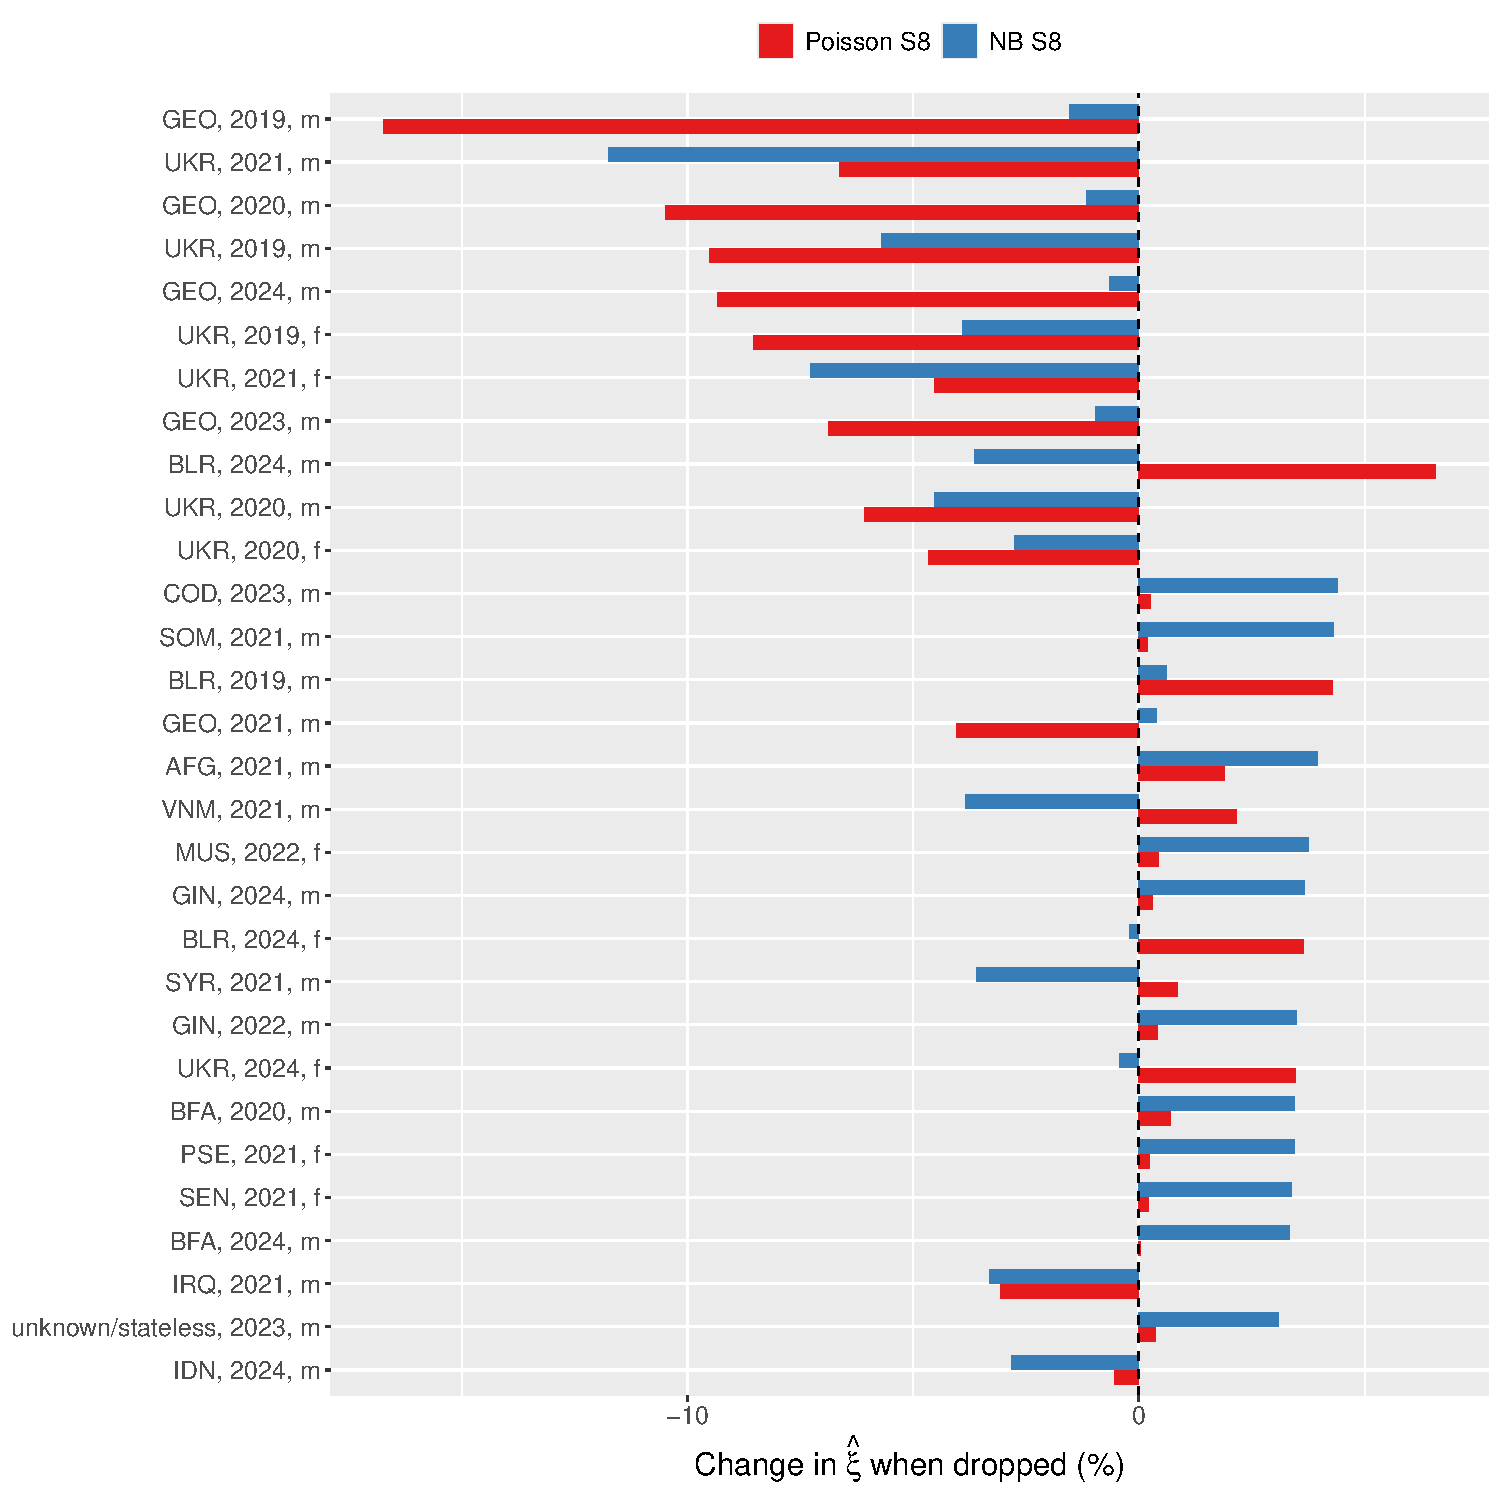
\includegraphics[width=0.9\textwidth]{figs-appen/figA-loo-obs.pdf}
    \caption{\label{fig-loo-obs}Observation-level LOO sensitivity (S8),
top 30 cells. Under Poisson, influence tracks $\mu$ (large cells
dominate); under NB, the variance function $V(\mu) = \mu + \mu^2/\theta$
caps large cells and lifts small-$\mu$ outliers.}
\end{figure}

Figure~\ref{fig-loo-obs} ranks individual cells by their influence on
$\hat\xi$. Under Poisson the leaders are Georgian and Ukrainian male
cells with high apprehension counts (e.g.\ Georgia 2019, $-17.5\%$).
Under NB the largest single cell is Ukraine 2021 ($-12.2\%$), but the
variance function down-weights the large Georgian cells (Georgia 2019
falls to $-1.4\%$) and lifts small-$\mu$ origins such as Congo,
Somalia, and Mauritius that carry almost no Poisson influence.
Figure~\ref{fig-loo-obs-scatter} plots the two rankings against each
other to make this asymmetry visible.

\begin{figure}[ht!]
    \centering
    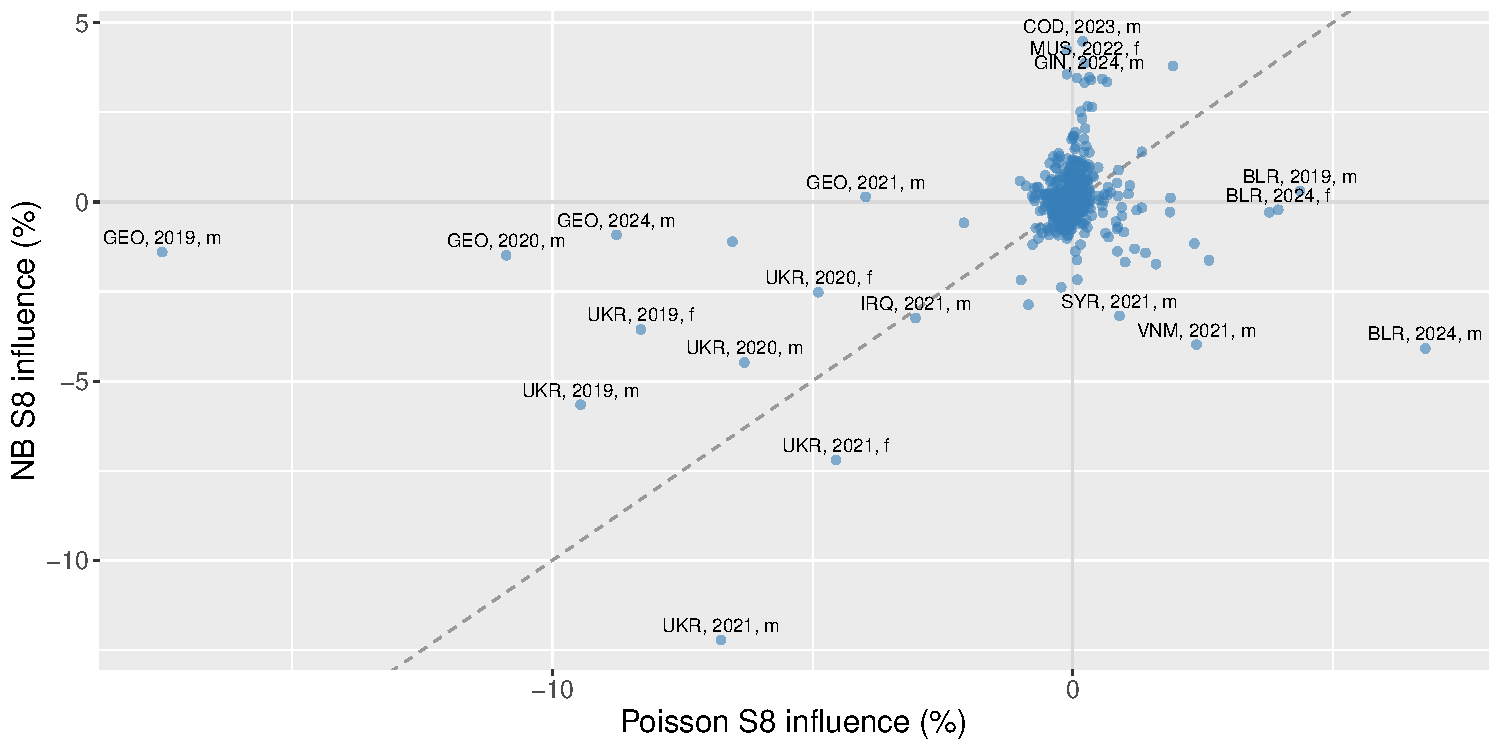
\includegraphics[width=0.9\textwidth]{figs-appen/figA-loo-obs-scatter.pdf}
    \caption{\label{fig-loo-obs-scatter}Observation-level LOO: Poisson vs
NB influence. Points off the diagonal are cells that affect the two
models asymmetrically; small-$\mu$ cells with high apprehension rates
sit in the upper-left (influential for NB, not Poisson), reflecting the
$\gamma$--$\theta$ confounding from the simulation study.}
\end{figure}

Under Poisson, the likelihood weight of cell $i$ scales with $\mu_i$,
so large cells (high $N$ and $m$) dominate. Under NB, the variance
function $V(\mu) = \mu + \mu^2/\theta$ caps the weight of high-$\mu$
cells and gives relatively more leverage to small-$\mu$ cells (low
$N$ but $m > 0$). This reflects the $\gamma$--$\theta$
confounding identified in the simulation study
(Section~\ref{sec-appendix-sim-study}): small-$\mu$ cells are where
$\gamma$ is hardest to separate from overdispersion.

\clearpage

\subsection{Anscombe residuals vs fitted values under S8}

\begin{figure}[ht!]
    \centering
    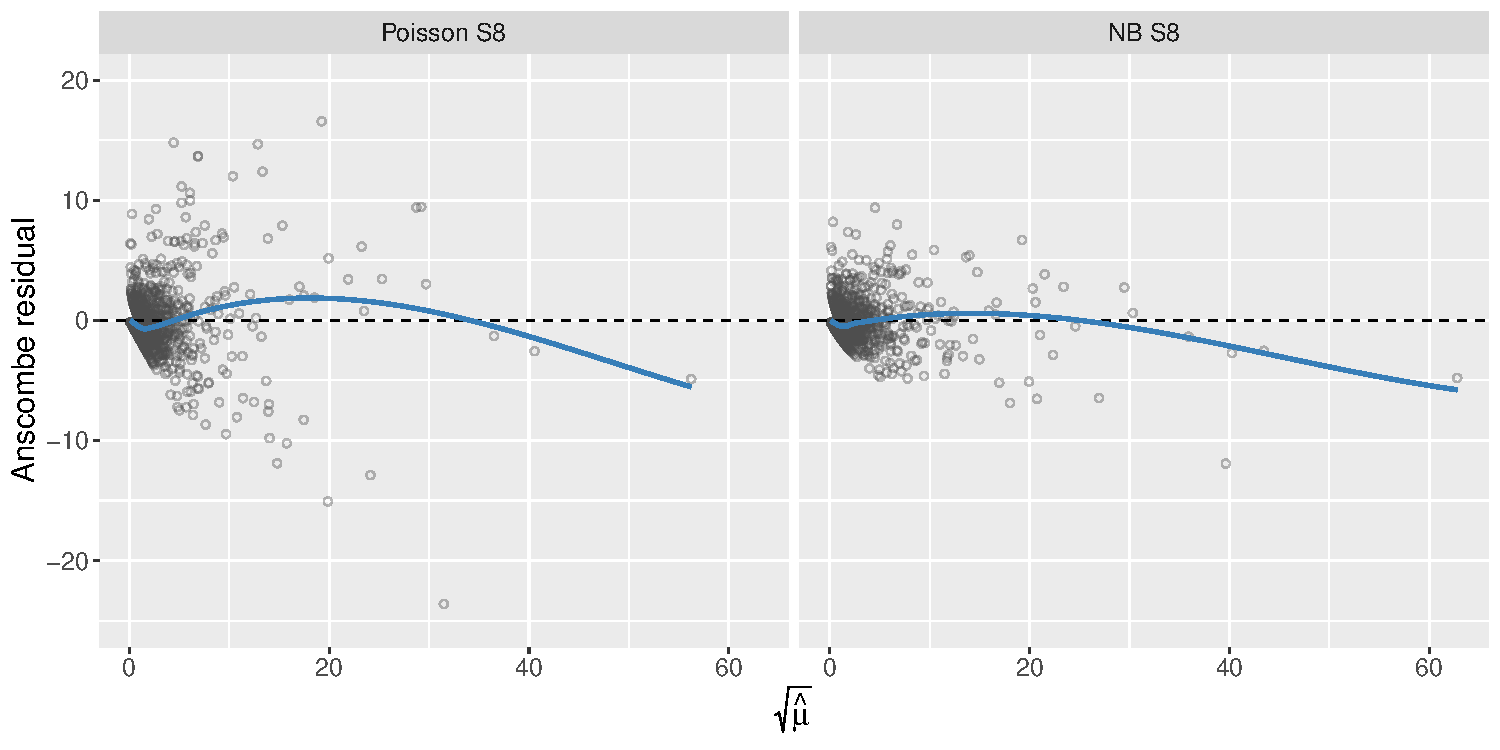
\includegraphics[width=0.9\textwidth]{figs-appen/figA-residuals.pdf}
    \caption{\label{fig-residuals}Anscombe residuals vs fitted values under S8}
\end{figure}

\clearpage

\subsection{Gamma profiles for S8}\label{gamma-profiles-for-s8}

\begin{figure}[ht!]
\centering
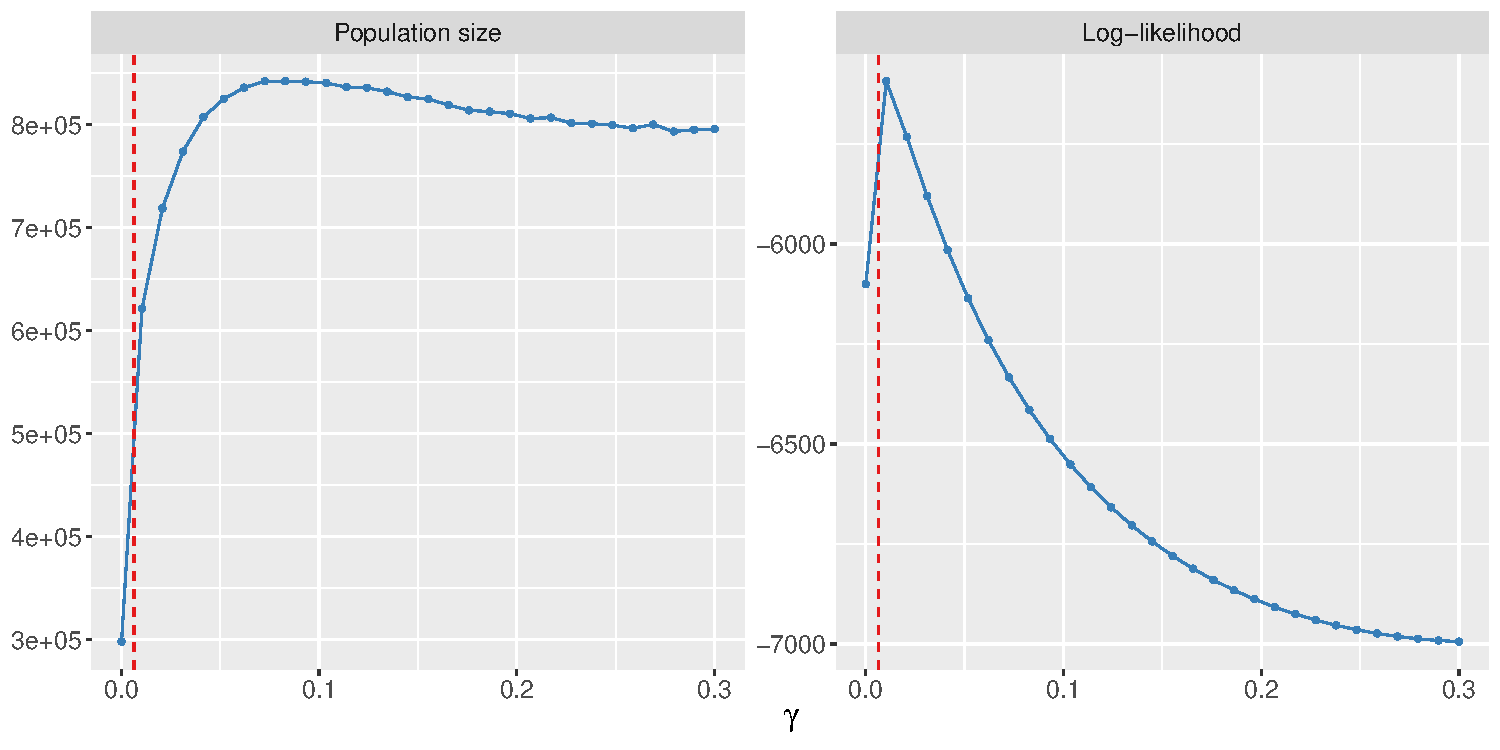
\includegraphics[width=0.9\textwidth]{figs-appen/figA-fig-gamma-profile-po.pdf}
\caption{\label{fig-gamma-profile-po}Poisson S8 gamma profile}
\end{figure}%

\begin{figure}[ht!]
\centering
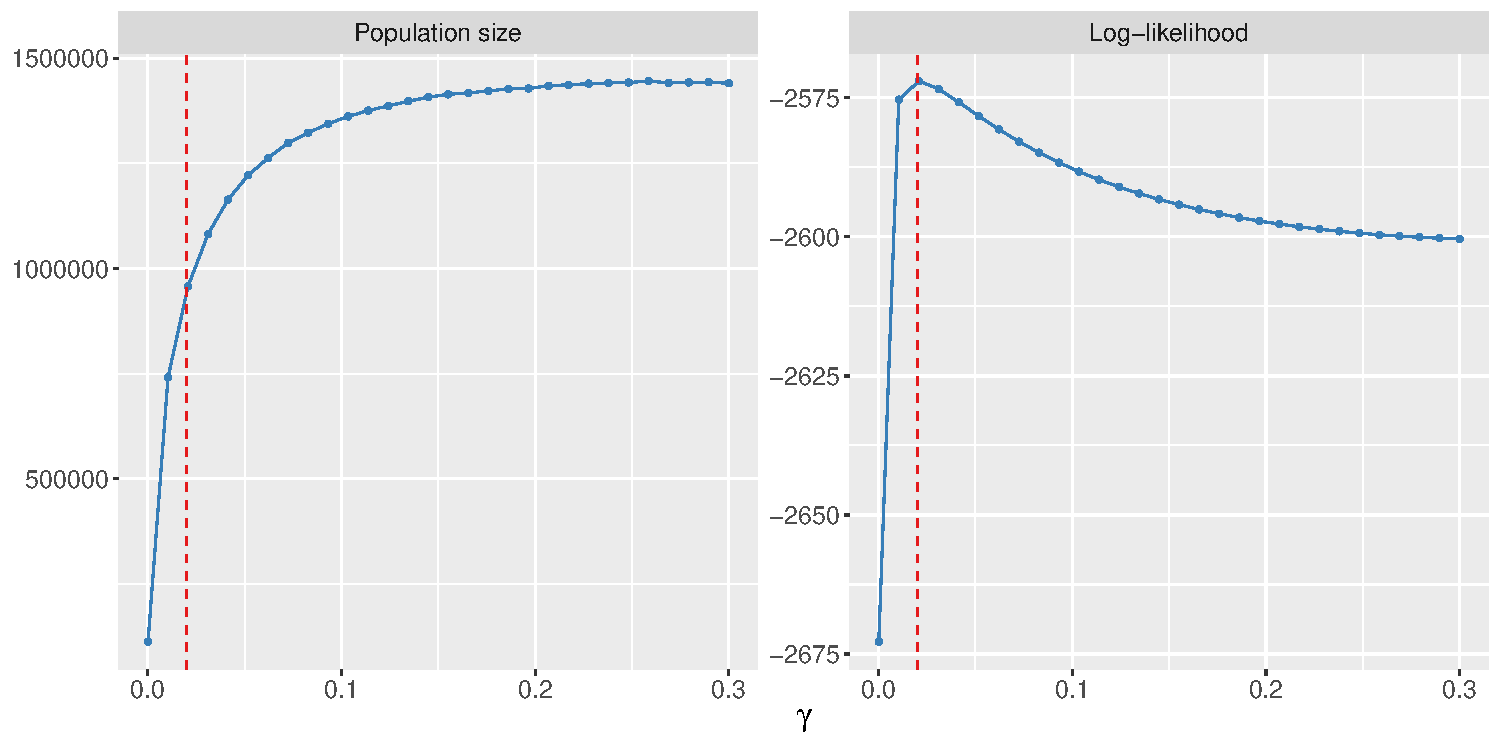
\includegraphics[width=0.9\textwidth]{figs-appen/figA-fig-gamma-profile-nb.pdf}
\caption{\label{fig-gamma-profile-nb}NB-MLE S8 gamma profile}
\end{figure}%

\clearpage

\subsection{Sensitivity to covariate-varying
gamma}\label{sec-appendix-cov-gamma}

The baseline specification uses a single estimated $\gamma$ for all
observations. We examine whether allowing $\gamma$ to vary by year,
sex, and/or Ukrainian origin improves fit, fixing
$\alpha = \text{year} \times \text{UKR} + \text{sex}$ and
$\beta = \text{year}$ (S8) and varying only the gamma specification.

\begin{table}[ht!]
\caption{\label{tbl-cov-gamma-aic}AIC and BIC by gamma specification and estimation method. All models use the S8 specification for alpha and beta with the ZUS reference population.} 
\fontsize{8.0pt}{10.0pt}\selectfont
\begin{tabular*}{\linewidth}{@{\extracolsep{\fill}}lrrrrrr}
\toprule
 & \multicolumn{3}{c}{{Poisson PMLE}} & \multicolumn{3}{c}{{NB-MLE}} \\ 
\cmidrule(lr){2-4} \cmidrule(lr){5-7}
$\gamma$ specification & AIC & BIC & $k\_\gamma$ & AIC & BIC & $k\_\gamma$ \\ 
\midrule\addlinespace[2.5pt]
constant & 11,535.6 & 11,640.2 & 1 & 5,265.2 & 5,375.0 & 1 \\ 
$\gamma \sim \text{year}$ & 11,313.6 & 11,444.3 & 6 & 5,260.1 & 5,396.1 & 6 \\ 
$\gamma \sim \text{sex}$ & 11,526.0 & 11,635.9 & 2 & 5,265.7 & 5,380.8 & 2 \\ 
$\gamma \sim \text{UKR}$ & 11,512.1 & 11,622.0 & 2 & 5,267.0 & 5,382.1 & 2 \\ 
$\gamma \sim \text{year} + \text{UKR}$ & 11,278.7 & 11,414.7 & 12 & 5,262.1 & 5,403.3 & 12 \\ 
$\gamma \sim \text{year} + \text{sex}$ & 11,142.6 & 11,278.6 & 12 & 5,259.8 & 5,401.0 & 12 \\ 
$\gamma \sim \text{year} + \text{sex} + \text{UKR}$ & 11,095.8 & 11,237.1 & 24 & 5,261.8 & 5,408.3 & 24 \\ 
\bottomrule
\end{tabular*}
\begin{minipage}{\linewidth}
\vspace{.05em}
Note: S8 specification: $\alpha \sim \text{year} \times \text{UKR} + \text{sex}$, $\beta \sim \text{year}$. ZUS reference population. $k\_\gamma$ = number of gamma parameters. Lower AIC/BIC is better.\\
\end{minipage}
\end{table}

Letting $\gamma$ vary by covariates improves the Poisson fit
substantially ($\Delta$AIC $\approx 440$ for $\gamma$ by year, sex
and Ukrainian origin) but barely changes the Negative Binomial
($\Delta$AIC $\approx 3$). This is the $\gamma$--$\theta$
trade-off: under NB, the dispersion parameter $\theta$ already absorbs
the detection heterogeneity that covariate-varying $\gamma$ captures
under Poisson. The NB $\theta$ stays close to $1.43$ across all gamma
specifications, so $\gamma$ and $\theta$ act as substitutes.

\begin{figure}[ht!] 
      \centering
      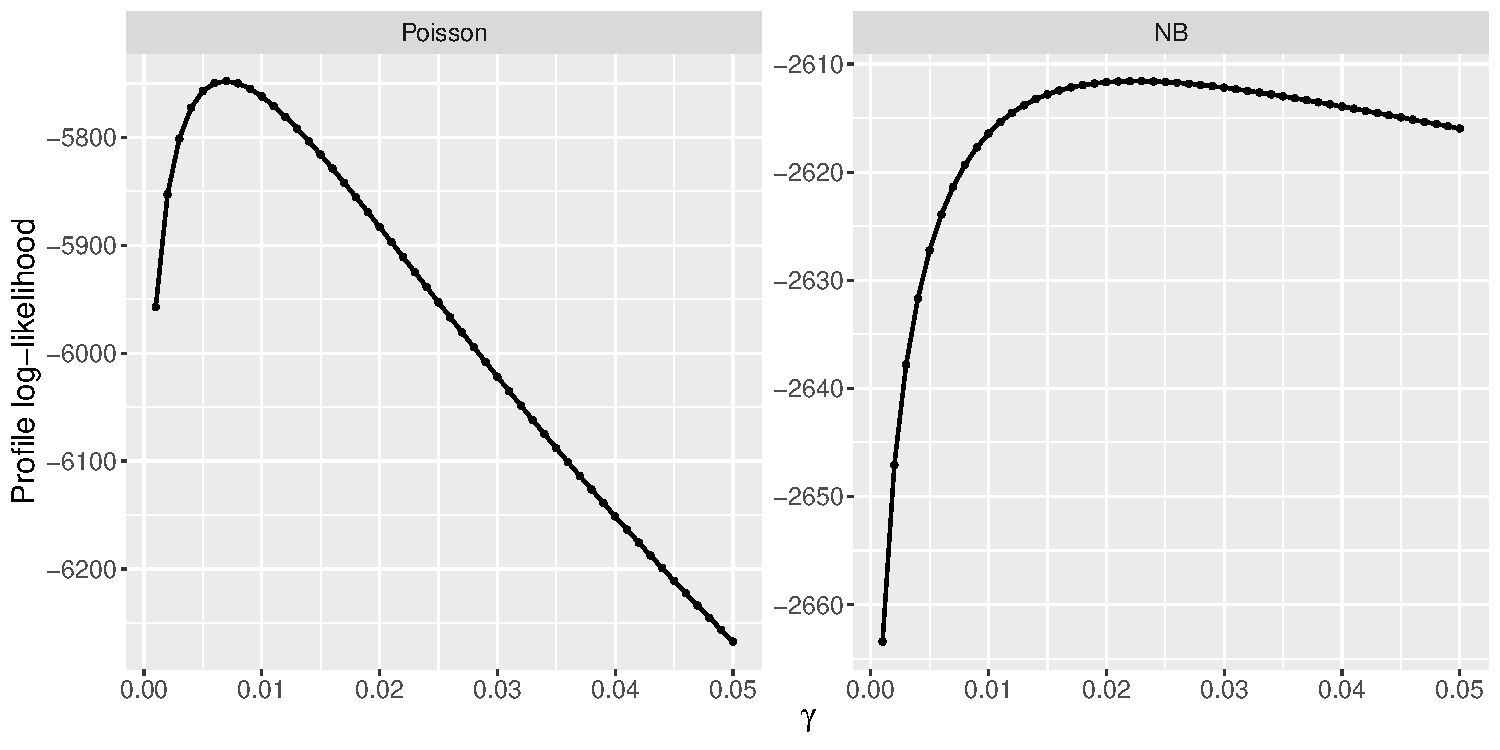
\includegraphics[width=0.9\textwidth]{figs-appen/figA-cov-gamma-profile.pdf}
      \caption{\label{fig-cov-gamma-profile}Profile log-likelihood of the
constant $\gamma$: Poisson (left, sharp peak) vs NB (right, flat). The
flat NB profile reflects weak identification from $\gamma$--$\theta$
confounding.}
\end{figure}

\begin{figure}[ht!]
    \centering
    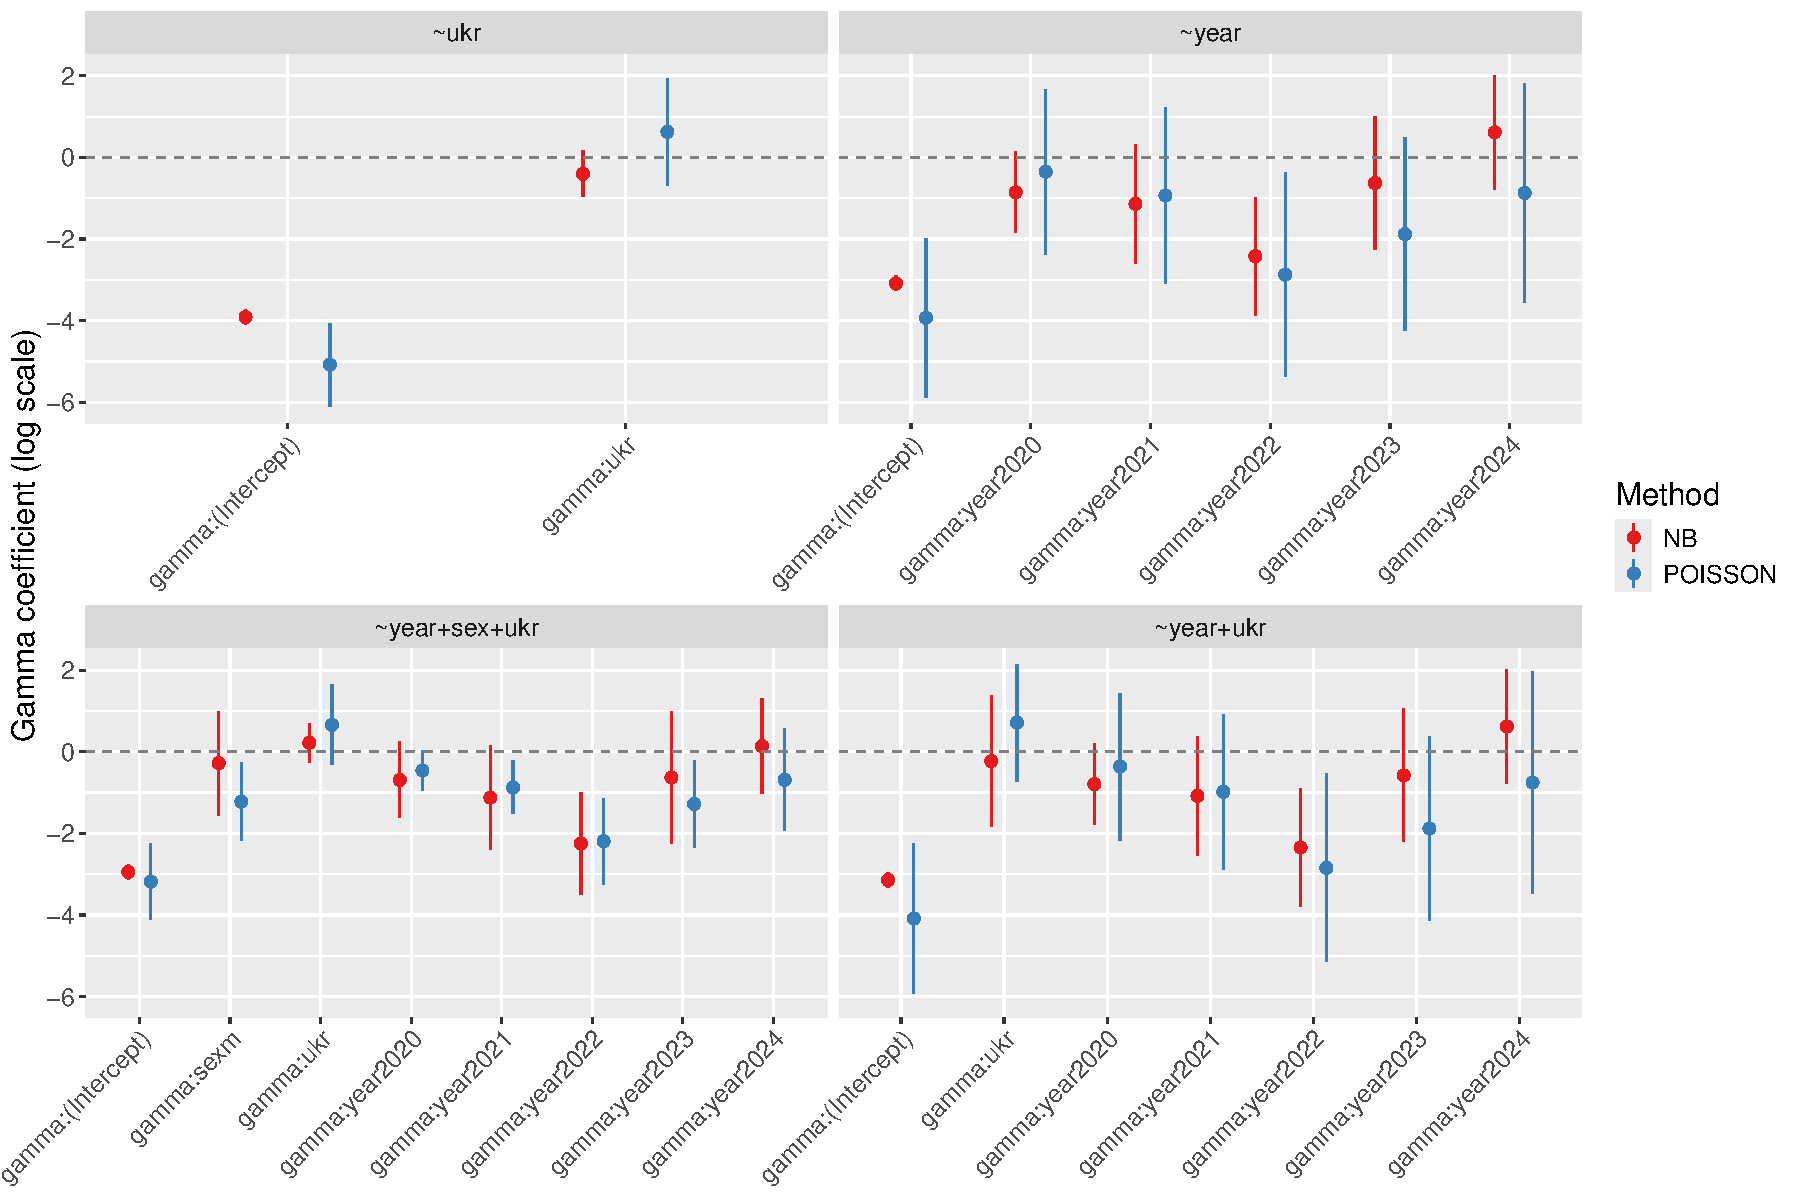
\includegraphics[width=0.9\textwidth]{figs-appen/figA-cov-gamma-coefs.pdf}
    \caption{\label{fig-cov-gamma-coefs}Gamma coefficients (log scale)
with 95\% Wald CIs. Under NB the intervals are wide and include zero,
reflecting weak identification.} 
\end{figure}

\begin{figure}[ht!]
    \centering
    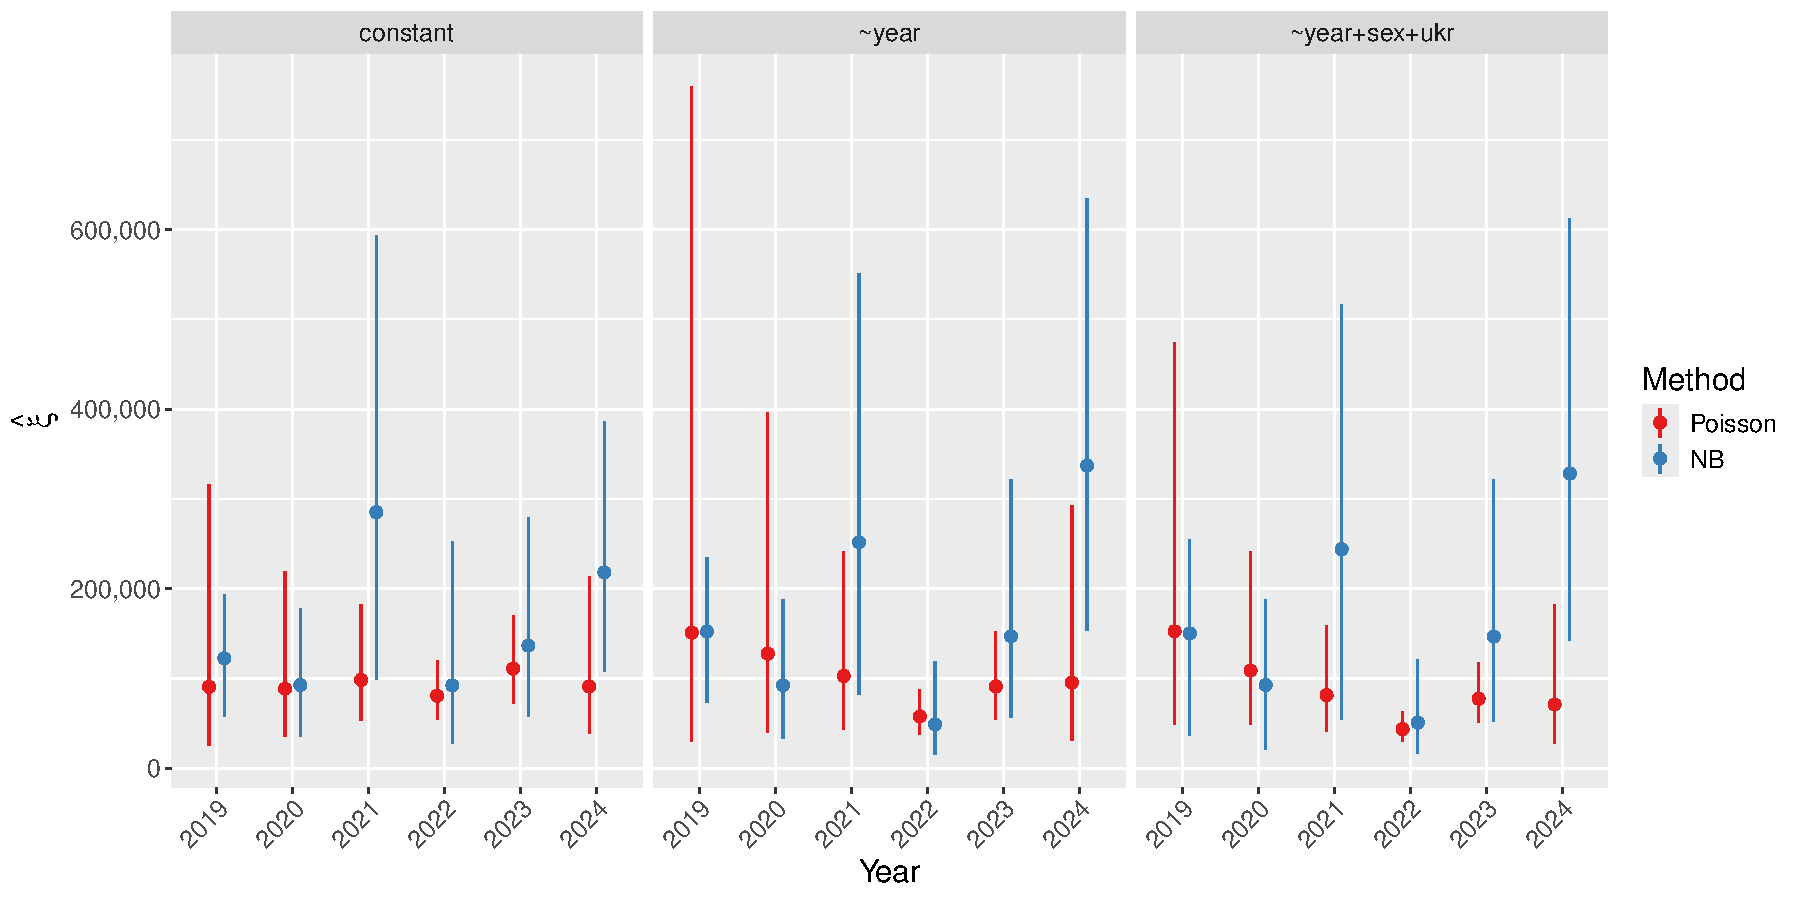
\includegraphics[width=0.9\textwidth]{figs-appen/figA-cov-gamma-popsize.pdf}
    \caption{\label{fig-cov-gamma-popsize}Estimated unauthorised
population by year: constant vs covariate-varying $\gamma$
(delta-method 95\% CI). The covariate-varying estimates fall within the
bootstrap intervals of the baseline model.}
\end{figure}

\begin{figure}[ht!]
    \centering
    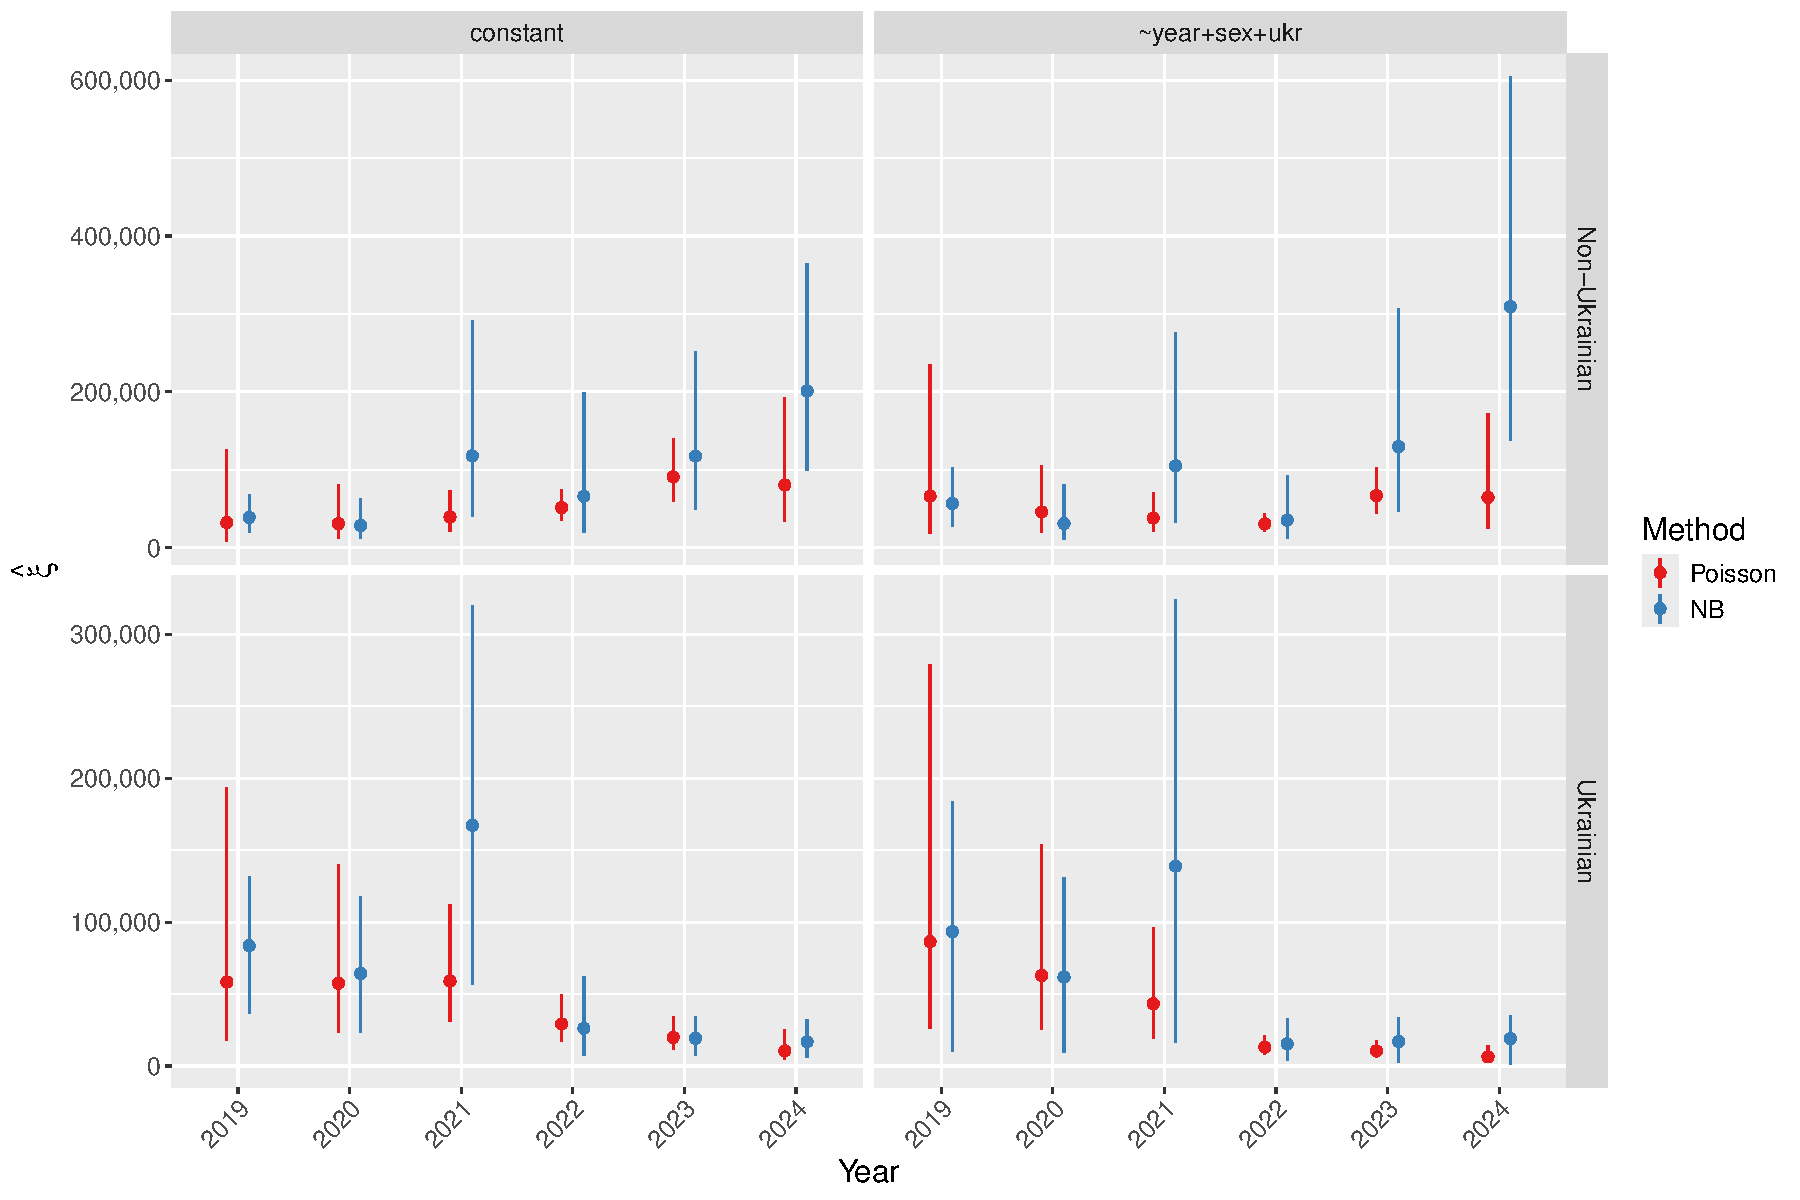
\includegraphics[width=0.9\textwidth]{figs-appen/figA-cov-gamma-popsize-ukr.pdf}
    \caption{\label{fig-cov-gamma-popsize-ukr}Estimated unauthorised
population by Ukrainian status: constant vs covariate-varying
$\gamma$ (delta-method 95\% CI).}
\end{figure}
  
We keep constant $\gamma$ in the main results because it is
parsimonious and well-identified under Poisson, leaves the NB fit (and
hence the Poisson--NB comparison) unchanged, and the resulting changes
in population size fall within the bootstrap intervals.

  
\clearpage

\subsection{Profile log-likelihood of $\alpha$ and $\beta$}\label{sec-appendix-profile-alpha-beta}

 To assess identification of the structural parameters $\alpha$ and
  $\beta$ under both Poisson and NB, we compute concentrated profile
  log-likelihoods with \texttt{uncounted::profile\_alpha()} and
  \texttt{uncounted::profile\_beta()}, varying each intercept over a grid
  while holding the other coefficients at their MLE.
  
  \begin{figure}[ht!]
      \centering
      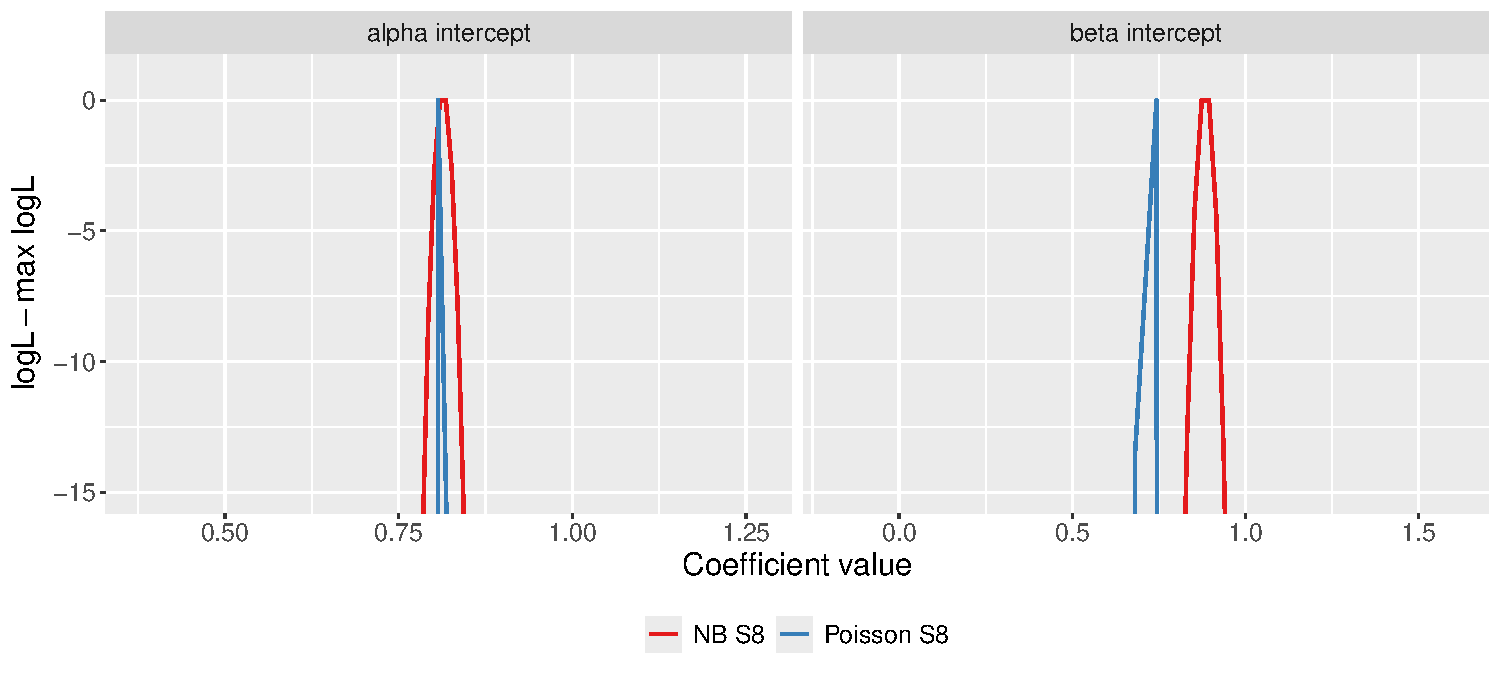
\includegraphics[width=0.9\textwidth]{figs-appen/figA-profile-alpha-beta.pdf}
      \caption{\label{fig-profile-alpha-beta}Concentrated profile
  log-likelihood of the $\alpha$ intercept (left) and $\beta$
  intercept (right) under Poisson S8 and NB S8. Both parameters are
  sharply identified under both models, unlike $\gamma$, whose NB
  profile is flat (see main text).}
  \end{figure}

  Both $\alpha$ and $\beta$ intercepts are sharply identified under
  Poisson and NB, with profile curvatures of similar magnitude. This
  contrasts with $\gamma$, whose NB profile is essentially flat. The
  $\gamma$--$\theta$ confounding is therefore specific to the
  baseline-detection parameter and does not extend to the structural
  community-anchor and exposure-elasticity parameters.

\clearpage

\section{Simulation studies}\label{sec-appendix-sim-study}

We conduct two simulation studies to assess the finite-sample properties
of the $\hat\xi$ estimator under known data-generating processes
(DGPs). The summary in Section~\ref{sec-simulation} gives the main
structure; here we report the full parameter values and the calibration
procedure, along with both simulation studies in detail.

\subsection{Data-generating process}\label{sec-appendix-sim-dgp}

For each replicate the simulator draws $C = 100$ communities and
proceeds in three stages.

\textbf{Stage 1: reference population.} Each community $i$ is assigned
a reference population size $N_i$ drawn from \[
N_i \sim \text{LogNormal}(\mu_N = 5.5, \, \sigma_N = 2.75), \quad N_i \geq 3,
\] with the lower truncation at 3 to avoid degenerate small-$N$ cases.
The lognormal parameters are chosen so that the simulated distribution
of $\log N_i$ matches the empirical distribution of $\log N_{it}$ in
the 2024 Polish ZUS panel.

\textbf{Stage 2: auxiliary count.} Given $N_i$, the auxiliary count
$n_i$ is drawn from a count-regression model with log-linear mean \[
\log \text{E}(n_i \mid N_i) = c_0 + c_1 \log N_i,
\] under either Poisson ---
$n_i \sim \text{Poisson}(\exp(c_0 + c_1 \log N_i))$ --- or Negative
Binomial  ---
$n_i \sim \text{NB}(\text{mean} = \exp(c_0 + c_1 \log N_i), \text{size} = \phi_n)$ distribution.
The intercept and slope are calibrated to the empirical Police-on-ZUS
regression in 2024:

{\def\LTcaptype{none} % do not increment counter
\begin{longtable}[]{@{}lll@{}}
\toprule\noalign{}
Parameter & Poisson DGP & Negative Binomial DGP \\
\midrule\noalign{}
\endhead
\bottomrule\noalign{}
\endlastfoot
Intercept $c_0$ & $-3.8073$ & $-4.0507$ \\
Slope $c_1$ & $0.9226$ & $0.9397$ \\
Dispersion $\phi_n$ & --- & $1.887$ \\
\end{longtable}
}

The slopes are close to one because the Police-on-ZUS relationship is
approximately proportional in the 2024 cross-section; the small
differences across the two DGPs reflect that the Poisson and NB
calibrations are fit separately to the same data.

\textbf{Stage 3: observed count.} Given $N_i$ and $n_i$, the
observed apprehension count $m_i$ follows the same power-law mean
structure that the estimators target: \[
\text{E}(m_i \mid N_i, n_i) = N_i^{\alpha} \left(\gamma + \frac{n_i}{N_i}\right)^{\beta}, \quad \alpha = 0.70, \, \beta = 0.50, \, \gamma = 0.005.
\] Again, $m_i$ is drawn under either Poisson ---
$m_i \sim \text{Poisson}(\mu_{m,i})$ --- or Negative Binomial
---
$m_i \sim \text{NB}(\text{mean} = \mu_{m,i}, \text{size} = \phi_m = 1.9229)$ distribution.
The structural parameters $(\alpha, \beta, \gamma)$ and the NB
dispersion $\phi_m$ are calibrated to the S8 fit on the 2024 Polish
ZUS panel (Poisson PML for $\alpha$, $\beta$, $\gamma$; NB for
$\phi_m$).

\textbf{DGP scenarios.} Crossing the two distributions for $n$
and $m$ yields four scenarios: Po($n$)--Po($m$),
Po($n$)--NB($m$), NB($n$)--Po($m$), NB($n$)--NB($m$).
Po($n$)--Po($m$) is the correctly specified case for Poisson PML;
NB($n$)--NB($m$) is the correctly specified case for NB. The mixed
scenarios test robustness to misspecification in one of the two count
distributions.

\textbf{Estimators.} Six estimators are run: OLS (on the log-linearised
model), NLS, Poisson PML (unconstrained and constrained to
$\alpha \in (0,1)$), and NB (unconstrained and constrained). Poisson
PML requires only correct specification of $\text{E}(m \mid X)$ and is
consistent regardless of the true variance function
\citep{SantosSilvaTenreyro2006}. NB additionally specifies
$\text{Var}(m \mid X) = \mu + \mu^2/\theta$, which can improve
efficiency under overdispersion but introduces a dispersion parameter
$\theta$ that confounds with the baseline exposure $\gamma$. NLS
results are reported in full here for completeness but are omitted from
the main-text summary tables because the estimator fails to converge (or
returns degenerate estimates) under NB-generated data.

\textbf{Replications.} Each of the four scenarios is replicated
$R = 2{,}000$ times with independent draws of
$(N_1, \dots, N_C, n_1, \dots, n_C, m_1, \dots, m_C)$. The
bias-correction analysis (see Section~\ref{sec-appendix-ommited-proofs})
and bootstrap CI comparison (see below) use $R_{\text{boot}} = 499$
bootstrap replicates per simulation replicate.


\clearpage

\subsection{Simulation 1: effect of aggregation}\label{sec-appendix-sim1}


In the first simulation ($R = 2{,}000$ replications, $C = 100$ countries
per replicate) we aggregate the countries that violate the positivity
condition ($n > 0$, $m > 0$, $n/N < 1$) into a single ``rest'' group,
which tests the aggregation procedure described in the main text.


\begin{table}[ht!]
\caption{\label{tbl-sim1}Simulation 1: bias, RMSE, coverage and CI width across four DGP scenarios under aggregation (all $m>0$, $n>0$). Analytical (delta-method) CIs. $R = 2{,}000$ replications.} 
\fontsize{8.0pt}{9.0pt}\selectfont
\begin{tabular*}{\linewidth}{@{\extracolsep{\fill}}lrrrrrr}
\toprule
Model & Bias (\%) & Bias BC (\%) & RMSE & Coverage (\%) & CI width (\%) & $R_{\text{ok}}$ \\ 
\midrule\addlinespace[2.5pt]
\multicolumn{7}{l}{NB($n$)-NB($m$)} \\[2.5pt] 
\midrule\addlinespace[2.5pt]
NB & -31.1 & -39.0 & 19,604 & 70.6 & 112.5 & 1950 \\ 
NB (c) & -31.1 & -38.2 & 19,605 & 70.9 & 113.4 & 1950 \\ 
NLS & -47.9 & -53.3 & 21,494 & 81.8 & 766.4 & 1950 \\ 
OLS & -34.0 & -43.9 & 20,499 & 74.4 & 127.2 & 1950 \\ 
Poisson & 11.6 & 11.2 & 103,375 & 79.6 & 253.3 & 1950 \\ 
Poisson (c) & 11.4 & 4998.1 & 101,745 & 79.5 & 253.5 & 1950 \\ 
\midrule\addlinespace[2.5pt]
\multicolumn{7}{l}{NB($n$)-Po($m$)} \\[2.5pt] 
\midrule\addlinespace[2.5pt]
NB & -39.9 & -40.7 & 21,184 & 40.9 & 57.8 & 1292 \\ 
NB (c) & -39.9 & -40.7 & 21,184 & 41.2 & 57.8 & 1292 \\ 
NLS & -34.5 & -34.7 & 8,897 & 56.6 & 66.7 & 1292 \\ 
OLS & -21.8 & -24.9 & 12,835 & 83.0 & 82.4 & 1292 \\ 
Poisson & -31.6 & -31.9 & 16,643 & 46.4 & 52.1 & 1292 \\ 
Poisson (c) & -31.6 & -31.8 & 16,643 & 46.5 & 52.1 & 1292 \\ 
\midrule\addlinespace[2.5pt]
\multicolumn{7}{l}{Po($n$)-NB($m$)} \\[2.5pt] 
\midrule\addlinespace[2.5pt]
NB & -15.8 & -26.6 & 20,216 & 82.7 & 144.1 & 1974 \\ 
NB (c) & -15.8 & -25.4 & 20,219 & 82.7 & 145.8 & 1974 \\ 
NLS & -32.9 & -47.9 & 26,258 & 83.9 & 4587.2 & 1971 \\ 
OLS & -17.6 & -30.6 & 21,171 & 87.1 & 160.0 & 1974 \\ 
Poisson & 155.0 & 153.5 & 1,368,824 & 83.4 & 490.3 & 1974 \\ 
Poisson (c) & 103.3 & 24749.5 & 218,537 & 82.8 & 481.5 & 1974 \\ 
\midrule\addlinespace[2.5pt]
\multicolumn{7}{l}{Po($n$)-Po($m$)} \\[2.5pt] 
\midrule\addlinespace[2.5pt]
NB & -2.1 & -2.8 & 7,752 & 93.5 & 47.4 & 1465 \\ 
NB (c) & -2.1 & -2.7 & 7,752 & 93.4 & 47.5 & 1465 \\ 
NLS & 9.3 & 9.0 & 3,612 & 92.2 & 86.2 & 1465 \\ 
OLS & 7.7 & 3.8 & 11,130 & 96.1 & 116.0 & 1465 \\ 
Poisson & -0.4 & -1.0 & 7,599 & 95.7 & 54.2 & 1465 \\ 
Poisson (c) & -0.4 & -0.9 & 7,599 & 95.7 & 54.3 & 1465 \\ 
\bottomrule
\end{tabular*}
\begin{minipage}{\linewidth}
\vspace{.05em}
Note: bias and CI width as a percentage of true $\xi$; RMSE on the original scale; coverage is the share of replications whose 95\% analytical CI contains $\xi$; $R_{\text{ok}}$ is the number of finite replications out of 2,000. NLS bias, bias BC and RMSE use median-based summaries (root-median-squared error) because a few replicates are numerically extreme under NB-generated data; the other estimators use mean-based summaries.\\
\end{minipage}
\end{table}


Under the correctly specified scenario Po($n$)-Po($m$), the Poisson estimator
is essentially unbiased ($-0.4\%$) with near-nominal coverage ($95.7\%$).
Under the misspecified NB($n$)-NB($m$) scenario it shows moderate positive
bias (about $12\%$) but keeps reasonable coverage (about $80\%$). The NB
estimator is biased downward under aggregation (about $-31\%$), because
the ``rest'' group absorbs small-country variation, and OLS is
substantially biased downward (about $-34\%$) through the $\log(m+1)$
transformation. NLS is numerically unstable under NB-generated data, so
its bias and RMSE in Table~\ref{tbl-sim1} use median-based summaries (see
the note); even so, it shows large negative bias under NB($n$)-NB($m$) and
Po($n$)-NB($m$). The mixed scenario NB($n$)-Po($m$) is the most challenging for
all estimators: Poisson shows $-31.6\%$ bias and only $46\%$ coverage,
reflecting the effect of overdispersed auxiliary counts on the detection
rate.

\clearpage

\subsection{Simulation 2: zeros in the counts}\label{sec-appendix-sim2}

The second simulation allows zeros in both $m$ and $n$ (no aggregation),
testing the ability of the $\gamma$ offset to handle sparse data.
Bootstrap confidence intervals ($R_{\text{boot}} = 499$, no clustering)
are also computed.


\begin{table}[ht!]
\caption{\label{tbl-sim2-analytical}Simulation 2: bias, RMSE, coverage and CI width with zeros allowed ($\gamma$ estimated). Analytical CIs. $R = 2{,}000$ replications.} 
\fontsize{7.0pt}{8.0pt}\selectfont
\begin{tabular*}{\linewidth}{@{\extracolsep{\fill}}lrrrrrrr}
\toprule
Model & Bias (\%) & Bias BC (\%) & Bias med (\%) & RMSE & Coverage (\%) & CI width (\%) & $R_{\text{ok}}$ \\ 
\midrule\addlinespace[2.5pt]
\multicolumn{8}{l}{NB($n$)-NB($m$)} \\[2.5pt] 
\midrule\addlinespace[2.5pt]
NB & 10.9 & -0.6 & 10.0 & 24,405 & 91.8 & 178.6 & 2000 \\ 
NB (c) & 10.9 & 1.2 & 10.0 & 24,418 & 91.4 & 181.2 & 2000 \\ 
NLS & -7.6 & -21.9 & -5.0 & 27,405 & 89.2 & 4599.0 & 1979 \\ 
OLS & -80.5 & -81.6 & -80.8 & 35,348 & 0.0 & 27.3 & 2000 \\ 
Poisson & 70.6 & 69.8 & 56.5 & 144,046 & 88.2 & 422.5 & 2000 \\ 
Poisson (c) & 66.4 & 74.8 & 55.4 & 117,479 & 88.0 & 420.4 & 2000 \\ 
\midrule\addlinespace[2.5pt]
\multicolumn{8}{l}{NB($n$)-Po($m$)} \\[2.5pt] 
\midrule\addlinespace[2.5pt]
NB & 0.8 & 0.3 & 0.9 & 4,412 & 91.8 & 34.7 & 2000 \\ 
NB (c) & 0.9 & 0.4 & 0.8 & 4,418 & 91.8 & 34.7 & 2000 \\ 
NLS & 0.4 & 0.2 & 0.6 & 2,896 & 94.4 & 79.0 & 1984 \\ 
OLS & -75.2 & -75.7 & -75.3 & 32,577 & 0.0 & 23.2 & 2000 \\ 
Poisson & 0.8 & 0.3 & 0.8 & 4,392 & 95.7 & 42.1 & 2000 \\ 
Poisson (c) & 0.8 & 0.4 & 0.8 & 4,392 & 95.7 & 42.1 & 2000 \\ 
\midrule\addlinespace[2.5pt]
\multicolumn{8}{l}{Po($n$)-NB($m$)} \\[2.5pt] 
\midrule\addlinespace[2.5pt]
NB & 6.9 & -4.7 & 5.4 & 20,226 & 92.8 & 178.8 & 2000 \\ 
NB (c) & 6.9 & -2.9 & 5.4 & 20,222 & 92.8 & 181.5 & 2000 \\ 
NLS & -41.2 & -62.0 & -40.4 & 25,595 & 84.6 & 3000.4 & 1980 \\ 
OLS & -77.9 & -79.0 & -78.3 & 33,975 & 0.2 & 28.2 & 2000 \\ 
Poisson & 77.8 & 76.3 & 53.5 & 534,916 & 83.7 & 392.2 & 2000 \\ 
Poisson (c) & 63.5 & 64.4 & 50.2 & 165,647 & 83.8 & 391.3 & 2000 \\ 
\midrule\addlinespace[2.5pt]
\multicolumn{8}{l}{Po($n$)-Po($m$)} \\[2.5pt] 
\midrule\addlinespace[2.5pt]
NB & -3.9 & -4.4 & -0.6 & 9,076 & 77.4 & 33.7 & 2000 \\ 
NB (c) & -0.3 & -0.7 & -0.6 & 3,465 & 93.1 & 34.7 & 2000 \\ 
NLS & -6.8 & -7.3 & -6.6 & 3,886 & 93.0 & 84.7 & 1997 \\ 
OLS & -70.3 & -70.9 & -70.7 & 31,600 & 0.0 & 22.9 & 2000 \\ 
Poisson & -0.4 & -0.9 & -0.7 & 3,899 & 95.1 & 40.3 & 2000 \\ 
Poisson (c) & -0.3 & -0.7 & -0.6 & 3,413 & 95.3 & 40.4 & 2000 \\ 
\bottomrule
\end{tabular*}
\begin{minipage}{\linewidth}
\vspace{.05em}
Note: bias and CI width as a percentage of true $\xi$; RMSE on the original scale. NLS bias, bias BC, bias med and RMSE use median-based summaries (root-median-squared error) under NB-generated data; other estimators use mean-based summaries.\\
\end{minipage}
\end{table}



\begin{table}[ht!]
\caption{\label{tbl-sim2-ci-comparison}Simulation 2: analytical vs bootstrap CI coverage and width, by scenario and estimator.} 
\fontsize{8.0pt}{9.0pt}\selectfont
\begin{tabular*}{\linewidth}{@{\extracolsep{\fill}}llrr}
\toprule
CI & Model & Coverage (\%) & CI width (\%) \\ 
\midrule\addlinespace[2.5pt]
\multicolumn{4}{l}{NB($n$)-NB($m$)} \\[2.5pt] 
\midrule\addlinespace[2.5pt]
Analytical & NB & 91.8 & 178.6 \\ 
Bootstrap & NB & 93.3 & 190.0 \\ 
Analytical & NB (c) & 91.4 & 181.2 \\ 
Bootstrap & NB (c) & 93.0 & 190.5 \\ 
Analytical & NLS & 89.2 & 4599.0 \\ 
Bootstrap & NLS & 65.9 & 1023.8 \\ 
Analytical & OLS & 0.0 & 27.3 \\ 
Bootstrap & OLS & 0.0 & 22.3 \\ 
Analytical & Poisson & 88.2 & 422.5 \\ 
Bootstrap & Poisson & 75.8 & 201.5 \\ 
Analytical & Poisson (c) & 88.0 & 420.4 \\ 
Bootstrap & Poisson (c) & 75.4 & 200.5 \\ 
\midrule\addlinespace[2.5pt]
\multicolumn{4}{l}{NB($n$)-Po($m$)} \\[2.5pt] 
\midrule\addlinespace[2.5pt]
Analytical & NB & 91.8 & 34.7 \\ 
Bootstrap & NB & 92.8 & 36.1 \\ 
Analytical & NB (c) & 91.8 & 34.7 \\ 
Bootstrap & NB (c) & 93.0 & 36.2 \\ 
Analytical & NLS & 94.4 & 79.0 \\ 
Bootstrap & NLS & 82.6 & 40.7 \\ 
Analytical & OLS & 0.0 & 23.2 \\ 
Bootstrap & OLS & 0.0 & 18.5 \\ 
Analytical & Poisson & 95.7 & 42.1 \\ 
Bootstrap & Poisson & 92.8 & 35.5 \\ 
Analytical & Poisson (c) & 95.7 & 42.1 \\ 
Bootstrap & Poisson (c) & 92.3 & 35.6 \\ 
\midrule\addlinespace[2.5pt]
\multicolumn{4}{l}{Po($n$)-NB($m$)} \\[2.5pt] 
\midrule\addlinespace[2.5pt]
Analytical & NB & 92.8 & 178.8 \\ 
Bootstrap & NB & 93.6 & 185.8 \\ 
Analytical & NB (c) & 92.8 & 181.5 \\ 
Bootstrap & NB (c) & 93.6 & 185.6 \\ 
Analytical & NLS & 84.6 & 3000.4 \\ 
Bootstrap & NLS & 60.8 & 670.7 \\ 
Analytical & OLS & 0.2 & 28.2 \\ 
Bootstrap & OLS & 0.0 & 24.1 \\ 
Analytical & Poisson & 83.7 & 392.2 \\ 
Bootstrap & Poisson & 71.8 & 193.6 \\ 
Analytical & Poisson (c) & 83.8 & 391.3 \\ 
Bootstrap & Poisson (c) & 71.8 & 193.3 \\ 
\midrule\addlinespace[2.5pt]
\multicolumn{4}{l}{Po($n$)-Po($m$)} \\[2.5pt] 
\midrule\addlinespace[2.5pt]
Analytical & NB & 77.4 & 33.7 \\ 
Bootstrap & NB & 92.8 & 36.4 \\ 
Analytical & NB (c) & 93.1 & 34.7 \\ 
Bootstrap & NB (c) & 92.6 & 35.7 \\ 
Analytical & NLS & 93.0 & 84.7 \\ 
Bootstrap & NLS & 87.2 & 52.0 \\ 
Analytical & OLS & 0.0 & 22.9 \\ 
Bootstrap & OLS & 0.0 & 19.7 \\ 
Analytical & Poisson & 95.1 & 40.3 \\ 
Bootstrap & Poisson & 92.8 & 36.1 \\ 
Analytical & Poisson (c) & 95.3 & 40.4 \\ 
Bootstrap & Poisson (c) & 93.1 & 35.5 \\ 
\bottomrule
\end{tabular*}
\begin{minipage}{\linewidth}
\vspace{.05em}
Note: coverage is the share of replications whose 95\% CI contains $\xi$; CI width is the median width as a percentage of $\xi$. Bootstrap CIs use $R_{\text{boot}} = 499$ per replicate without clustering. NLS CI widths can be very large under NB-generated scenarios.\\
\end{minipage}
\end{table}



\begin{table}[ht!]
\caption{\label{tbl-sim2-gamma}Simulation 2: recovery of $\gamma$ across scenarios and estimators. Median, mean, and the share of replications where $\hat\gamma$ hits the upper boundary ($\geq 0.49$). True $\gamma = 0.005$.} 
\fontsize{8.0pt}{9.0pt}\selectfont
\begin{tabular*}{\linewidth}{@{\extracolsep{\fill}}lrrrrr}
\toprule
Model & Median & Mean & Q75 & \% boundary & \% $>0.1$ \\ 
\midrule\addlinespace[2.5pt]
\multicolumn{6}{l}{NB($n$)-NB($m$)} \\[2.5pt] 
\midrule\addlinespace[2.5pt]
NB & 0.0048 & 0.0111 & 0.0102 & 0.1 & 1.2 \\ 
NB (c) & 0.0048 & 0.0113 & 0.0102 & 0.1 & 1.2 \\ 
NLS & 0.0386 & 0.1652 & 0.3558 & 3.8 & 45.3 \\ 
OLS & 0.0099 & 0.0678 & 0.0322 & 6.2 & 13.8 \\ 
Poisson & 0.0038 & 0.0545 & 0.0234 & 0.7 & 14.2 \\ 
Poisson (c) & 0.0039 & 0.0581 & 0.0241 & 1.9 & 14.4 \\ 
\midrule\addlinespace[2.5pt]
\multicolumn{6}{l}{NB($n$)-Po($m$)} \\[2.5pt] 
\midrule\addlinespace[2.5pt]
NB & 0.0050 & 0.0063 & 0.0061 & 0.1 & 0.2 \\ 
NB (c) & 0.0050 & 0.0053 & 0.0061 & 0.0 & 0.0 \\ 
NLS & 0.0050 & 0.0058 & 0.0066 & 0.0 & 0.1 \\ 
OLS & 0.0070 & 0.0153 & 0.0099 & 0.7 & 1.7 \\ 
Poisson & 0.0050 & 0.0053 & 0.0061 & 0.0 & 0.0 \\ 
Poisson (c) & 0.0050 & 0.0053 & 0.0061 & 0.0 & 0.0 \\ 
\midrule\addlinespace[2.5pt]
\multicolumn{6}{l}{Po($n$)-NB($m$)} \\[2.5pt] 
\midrule\addlinespace[2.5pt]
NB & 0.0045 & 0.0155 & 0.0112 & 0.2 & 2.9 \\ 
NB (c) & 0.0045 & 0.0156 & 0.0112 & 0.3 & 2.8 \\ 
NLS & 0.2770 & 0.2389 & 0.3602 & 7.7 & 73.0 \\ 
OLS & 0.0771 & 0.2112 & 0.4526 & 24.1 & 46.4 \\ 
Poisson & 0.0058 & 0.0619 & 0.0420 & 0.9 & 20.9 \\ 
Poisson (c) & 0.0042 & 0.0480 & 0.0224 & 2.5 & 12.0 \\ 
\midrule\addlinespace[2.5pt]
\multicolumn{6}{l}{Po($n$)-Po($m$)} \\[2.5pt] 
\midrule\addlinespace[2.5pt]
NB & 0.0060 & 0.1210 & 0.3063 & 16.2 & 26.2 \\ 
NB (c) & 0.0048 & 0.0083 & 0.0076 & 0.4 & 0.6 \\ 
NLS & 0.0084 & 0.0715 & 0.1963 & 0.1 & 31.8 \\ 
OLS & 0.0358 & 0.1422 & 0.2865 & 17.8 & 27.7 \\ 
Poisson & 0.0048 & 0.0073 & 0.0076 & 0.0 & 0.7 \\ 
Poisson (c) & 0.0048 & 0.0061 & 0.0075 & 0.0 & 0.1 \\ 
\bottomrule
\end{tabular*}
\begin{minipage}{\linewidth}
\vspace{.05em}
Note: boundary = $\hat\gamma \geq 0.49$ (upper optimisation bound). The unconstrained NB hits this boundary in 16\% of Po($n$)-Po($m$) replications, inflating $\hat\gamma$ by a factor of 24 relative to the true value.\\
\end{minipage}
\end{table}



With zeros allowed, OLS collapses (about $0\%$ coverage) because
$\log(m+1)$ attenuates the signal when most counts are small. NLS remains
numerically unstable under NB-generated data; under median-based
summaries it shows large negative bias under Po($n$)-NB($m$). Neither
log-linearised estimator is suitable for sparse count data.

Under the correctly specified scenario Po($n$)-Po($m$), the Poisson estimator
achieves $-0.4\%$ bias, RMSE of $3{,}899$, and $95.1\%$ coverage. Under
NB misspecification its bias rises to about $71$--$78\%$ as overdispersion
inflates the mean estimate, while coverage stays above $83\%$ through
wider CIs.

The NB estimator, which specifies $\text{Var}(m \mid X) = \mu +
\mu^2/\theta$, achieves $7$--$11\%$ bias with about $92\%$ coverage under
NB-generated data, against $71$--$78\%$ for Poisson. The cost is
$\gamma$--$\theta$ confounding: both $\theta$ and $\gamma$ absorb
variation beyond the Poisson mean, so $\gamma$ is weakly identified.
Table~\ref{tbl-sim2-gamma} shows that the unconstrained NB overestimates
$\gamma$ by a factor of 24 (mean $\hat\gamma = 0.12$ vs true $0.005$) in
$16\%$ of Po($n$)-Po($m$) replications, hitting the optimisation boundary.
RMSE rises from $3{,}413$ (Poisson constrained) to $9{,}076$ (NB
unconstrained). The constrained NB (NB$_c$, $\alpha \in (0,1)$) reduces
boundary hits to $0.4\%$ and RMSE to $3{,}465$, with $93\%$ coverage.

The multiplicative lognormal bias correction reduces NB bias from
$10.9\%$ to $-0.6\%$ under NB($n$)-NB($m$) and from $6.9\%$ to $-4.7\%$ under
Po($n$)-NB($m$); the bootstrap median tracks the bias-corrected estimate
closely.



\subsection{Summary of simulation findings}\label{sec-appendix-sim-summary}

The two simulation studies provide the following evidence for the
empirical analysis.

\begin{enumerate}
\item Poisson PMLE, which requires only a correct mean specification,
  gives stable $\hat\xi$ estimates across scenarios; even under
  NB-generated data its coverage stays at $80$--$88\%$ through wider CIs.
\item NB-MLE gains efficiency when correctly specified but introduces
  $\gamma$--$\theta$ confounding: $\theta$ absorbs variation otherwise
  attributed to $\gamma$, so the unconstrained NB overestimates $\gamma$
  by a factor of 24 in $16\%$ of Poisson-generated replications. The
  constrained NB ($\alpha \in (0,1)$) cuts boundary hits from $16\%$ to
  $0.4\%$ and is preferred when NB is used as a sensitivity check.
\item OLS with $\log(m+1)$ is severely biased when zeros are present
  (Simulation 2) and is unsuitable for sparse count data.
\item The multiplicative lognormal bias correction reduces NB bias from
  about $11\%$ to under $1\%$ under NB-generated data.
\item Bootstrap CIs are wider than the analytical (delta-method) CIs,
  particularly for NB. The empirical analysis uses a cluster bootstrap to
  account for within-country correlation.
\end{enumerate}


\clearpage

\section{OLS and NLS estimation details}\label{sec-appendix-ols-nls}

\textbf{OLS estimation.} The OLS estimator operates on the
log-linearised form of the model:

\begin{equation}\protect\phantomsection\label{eq-ols-model}{
\log(m_{it}) = \alpha \log N_{it} + \beta \log\left(\frac{n_{it}}{N_{it}}\right) + \epsilon_{it},
}\end{equation}

where $\alpha$ is the Community Anchor parameter and $\beta$ is the
Exposure Elasticity. The no-intercept specification follows directly
from the theoretical model
$\mu_{it} = N_{it}^\alpha (n_{it}/N_{it})^\beta$, which contains no
free multiplicative constant.

This specification requires $m_{it} > 0$ and $n_{it} > 0$. When
zeros are present, we either aggregate the data to eliminate zero cells
or add a small positive constant, e.g.~$m_{it}+1$ and a shift
parameter $\gamma > 0$ to the exposure ratio $n_{it}/N_{it}$ to
handle zero values. In simulation studies we verify the finite-sample
performance when the data are aggregated in such a way that
$m_{it} > 0$ and $n_{it} > 0$ (see
Section~\ref{sec-appendix-sim-study}). As expected, the OLS approach is
not well suited for sparse count data.

\textbf{NLS estimation.} The nonlinear least squares estimator operates
on the original scale:

\begin{equation}\protect\phantomsection\label{eq-nls-model}{
m_{it} = N_{it}^\alpha \left(\frac{n_{it}}{N_{it}}\right)^\beta + \epsilon_{it}.
}\end{equation}

We consider this model both with and without the $\gamma$ parameter,
and all parameters are estimated using the Levenberg--Marquardt
algorithm as implemented in the \emph{minpack.lm} package in R. Unlike
the count model estimators, NLS does not require distributional
assumptions beyond a mean specification, which makes it a useful
robustness check. However, in the simulation studies we find that the
model yields unbiased estimates of $\xi$ only when both $n$ and
$m$ follow a Poisson distribution.

\clearpage

\section{Omitted derivations}\label{sec-appendix-ommited-proofs}

\subsection{\texorpdfstring{OLS with unknown
$\gamma$}{OLS with unknown \textbackslash gamma}}\label{ols-with-unknown-gamma}

The OLS estimator operates on the log-linearised form of the model.
Given the specification $m_i = N_i^\alpha (\gamma + n_i/N_i)^\beta$,
taking logarithms yields

\[
\log(y_i) = \alpha \log N_i + \beta \log(\gamma + n_i/N_i) + \varepsilon_i,
\]

where $y_i = m_i$ when all counts are positive, and $y_i = m_i + 1$
when any $m_i = 0$ (to avoid $\log(0)$). The \texttt{uncounted}
package automatically selects the appropriate transformation based on
the data.

Since $\gamma$ enters the model non-linearly, estimation proceeds via
concentrated (profile) least squares. For a fixed value of $\gamma$,
the model is linear in $(\alpha, \beta)$ and can be estimated by
ordinary least squares. Define the profile sum of squared errors as

\[
S(\gamma) = \sum_{i=1}^{I} \left[ \log(y_i) - \hat{\alpha}(\gamma) \log N_i - \hat{\beta}(\gamma) \log(\gamma + n_i/N_i) \right]^2,
\]

where $\hat{\alpha}(\gamma)$ and $\hat{\beta}(\gamma)$ denote the
OLS coefficients conditional on $\gamma$. The estimator minimises
$S(\gamma)$ over the interval $\gamma \in (10^{-10}, 0.5)$ using a
multi-start grid search followed by Brent's method, yielding
$\hat{\gamma}$. The final estimates $\hat{\alpha}$ and
$\hat{\beta}$ are then obtained from the OLS regression evaluated at
$\hat{\gamma}$.

\subsection{Constrained estimation via logit
reparametrisation}\label{sec-appendix-constrained}

The theoretical model requires $\alpha \in (0,1)$ and $\beta > 0$.
The unconstrained estimators (Poisson PML, NB) estimate these parameters
on $\mathbb{R}$ and do not enforce the restrictions. We impose them
through link functions: the logit for $\alpha$ and the log for
$\beta$.

For observation $i$ with covariate vector $\mathbf{x}_i$, define the
linear predictor $\eta_i = \mathbf{x}_i' \boldsymbol{\eta}$ and set

\begin{equation}\protect\phantomsection\label{eq-constrained-link}{
\alpha_i = \text{logit}^{-1}(\eta_i) = \frac{1}{1 + \exp(-\eta_i)}, \qquad \beta = \exp(\zeta),
}\end{equation}

where $\boldsymbol{\eta}$ and $\zeta$ are the parameters to be
estimated (on $\mathbb{R}$). The log conditional mean becomes

\begin{equation}\protect\phantomsection\label{eq-constrained-logmu}{
\log(\mu_i) = \text{logit}^{-1}(\mathbf{x}_i' \boldsymbol{\eta}) \cdot \log N_i + \exp(\zeta) \cdot \log\!\left(\gamma + \frac{n_i}{N_i}\right).
}\end{equation}

The logit link makes $\log(\mu_i)$ non-linear in $\boldsymbol{\eta}$
even under the Poisson model, so estimation requires numerical
optimisation of the (pseudo) log-likelihood with respect to
$(\boldsymbol{\eta}, \zeta, \gamma)$. Starting values are obtained
from the unconstrained fit:
$\boldsymbol{\eta}_0 = \text{logit}(\hat{\boldsymbol{\alpha}}_{\text{unc}})$,
$\zeta_0 = \log(\hat{\beta}_{\text{unc}})$.

Coefficients are reported on the link scale ($\boldsymbol{\eta}$,
$\zeta$). Response-scale values
$\alpha_i = \text{logit}^{-1}(\mathbf{x}_i' \hat{\boldsymbol{\eta}})$
and $\beta = \exp(\hat\zeta)$ are obtained by applying the inverse
link. Standard errors on the response scale follow from the delta
method:

\begin{equation}\protect\phantomsection\label{eq-constrained-var-alpha}{
\text{Var}(\hat\alpha_i) \approx [\hat\alpha_i(1 - \hat\alpha_i)]^2 \cdot \mathbf{x}_i' \mathbf{V}_{\eta} \mathbf{x}_i,
}\end{equation}

where $\mathbf{V}_{\eta}$ is the variance-covariance matrix of
$\hat{\boldsymbol{\eta}}$ (model-based or HC-robust).

For the population size estimator
$\hat\xi = \sum_i N_i^{\hat\alpha_i}$, the gradient with respect to
$\boldsymbol{\eta}$ is

\begin{equation}\protect\phantomsection\label{eq-constrained-gradient}{
\frac{\partial \xi}{\partial \eta_j} = \sum_i N_i^{\alpha_i} \ln(N_i) \cdot \alpha_i(1 - \alpha_i) \cdot x_{ij}.
}\end{equation}

Confidence intervals for $\xi$ are constructed by forming a Wald
interval on the $\boldsymbol{\eta}$ scale and mapping it through the
monotone transformation
$g(\boldsymbol{\eta}) = \sum_i N_i^{\text{logit}^{-1}(\mathbf{x}_i' \boldsymbol{\eta})}$.

The multiplicative lognormal bias correction \eqref{eq-bias-correction}
in the main text does not apply under the logit link because
$N_i^{\text{logit}^{-1}(\eta_i)}$ is not an exponential function of
$\eta_i$. We use the second-order Taylor correction instead:

\begin{equation}\protect\phantomsection\label{eq-constrained-bc}{
\hat{\xi}^{\text{BC}} = \hat{\xi} - \frac{1}{2} \sum_{i=1}^{I} N_i^{\hat{\alpha}_i} [\ln(N_i)]^2 \cdot \text{Var}(\hat{\alpha}_i),
}\end{equation}

where $\text{Var}(\hat{\alpha}_i)$ includes the delta-method
adjustment \eqref{eq-constrained-var-alpha}. This correction can be
positive or negative depending on $\alpha_i$.

\subsection{\texorpdfstring{Bias correction for
$\hat{\xi}_{t}$}{Bias correction for \textbackslash hat\{\textbackslash xi\}\_\{t\}}}\label{bias-correction-for-hatxi_t}

Since $g(\alpha) = \sum_{i=1}^I N_{it}^\alpha$ is nonlinear in
$\alpha$, the plug-in estimator $\hat{\xi}_t = g(\hat{\alpha})$ is
biased. Moreover, $g$ is convex for $N_{it} > 1$, so Jensen's
inequality implies $\text{E}[\hat{\xi}_t] \geq \xi_t$ when
$\hat{\alpha}$ is unbiased.

\textbf{Second-order Taylor approximation.} A Taylor expansion of $g$
around the true $\alpha$ gives:

\begin{equation}\protect\phantomsection\label{eq-bias-approx}{
\text{Bias}[\hat\xi_t] \approx g'(\alpha) \cdot \text{Bias}[\hat\alpha] + \frac{1}{2} g''(\alpha) \cdot \left(\text{Var}[\hat\alpha] + \text{Bias}[\hat\alpha]^2\right),
}\end{equation}

where $g'(\alpha) = \sum_i N_i^\alpha \ln(N_i)$ and
$g''(\alpha) = \sum_i N_i^\alpha [\ln(N_i)]^2$. Assuming
$\hat\alpha$ is unbiased (consistent under correct mean specification
for Poisson PML), the first-order term vanishes and the Taylor bias
correction becomes:

\[
\hat\xi_t^{\text{Taylor}} = \hat\xi_t - \frac{1}{2} \sum_{i=1}^I N_{it}^{\hat\alpha_i} [\ln(N_{it})]^2 \cdot \mathbf{x}_i' \hat{\mathbf{V}}_{\text{model}} \mathbf{x}_i,
\]

where $\mathbf{x}_i$ is the $i$-th row of the $\alpha$ design
matrix and $\hat{\mathbf{V}}_{\text{model}}$ is the model-based
(homoscedastic) variance of $\hat\alpha$. This approximation has two
drawbacks: (i) it can produce negative bias-corrected estimates when
variance is large and $\sum N_i^{\alpha} (\ln N_i)^2$ is large
relative to $\hat{\xi}$; (ii) approximation error grows for
heavy-tailed $N$ distributions. In simulations, the Taylor correction
reduces bias by about 88\%.

\textbf{Multiplicative lognormal correction (recommended).} Since
$N_i^{\hat{\alpha}} = \exp(\hat{\alpha} \ln N_i)$ and
$\hat{\alpha} \sim N(\alpha, V)$, the moment generating function of
the normal distribution gives
$\text{E}[N_i^{\hat{\alpha}}] = N_i^{\alpha} \exp(\frac{1}{2} (\ln N_i)^2 V)$.
Inverting this yields:

\[
\hat{\xi}_t^{\text{BC}} = \sum_{i=1}^{I} N_{it}^{\hat{\alpha}} \exp\left(-\frac{1}{2} (\ln N_{it})^2 \, \mathbf{x}_i' \hat{\mathbf{V}} \mathbf{x}_i\right).
\]

This estimator is exact under normality of $\hat{\alpha}$, always
positive, and in simulations reduces bias by about 94\%. The
\texttt{uncounted} package uses this form as the default.

\textbf{Variance choice.} Both corrections use the model-based variance
rather than HC-robust variance, because the latter can be inflated by
high-leverage observations (e.g., Ukraine with $N > 400{,}000$),
leading to overcorrection. The model-based variance is computed as
$\hat{\mathbf{V}}_{\text{model}} = \hat\sigma^2 (\mathbf{X}'\mathbf{W}\mathbf{X})^{-1}$
for OLS/NLS, or $(\mathbf{X}'\mathbf{W}\mathbf{X})^{-1}$ for
Poisson/NB (where $\mathbf{W}$ is the working weight matrix).

For constrained models, the delta method accounts for the logit link
\eqref{eq-constrained-var-alpha} and the Taylor correction
\eqref{eq-constrained-bc} replaces the lognormal form; see
Section~\ref{sec-appendix-constrained}.
